\documentclass[final,5p,times,twocolumn,authoryear]{elsarticle} %review=doublespace preprint=single 5p=2 column
%%% Begin My package additions %%%%%%%%%%%%%%%%%%%
\usepackage[hyphens]{url}

  \journal{Atmospheric Research} % Sets Journal name


\usepackage{lineno} % add
\providecommand{\tightlist}{%
  \setlength{\itemsep}{0pt}\setlength{\parskip}{0pt}}

\usepackage{graphicx}
\usepackage{booktabs} % book-quality tables
%%%%%%%%%%%%%%%% end my additions to header

\usepackage[T1]{fontenc}
\usepackage{lmodern}
\usepackage{amssymb,amsmath}
\usepackage{ifxetex,ifluatex}
\usepackage{fixltx2e} % provides \textsubscript
% use upquote if available, for straight quotes in verbatim environments
\IfFileExists{upquote.sty}{\usepackage{upquote}}{}
\ifnum 0\ifxetex 1\fi\ifluatex 1\fi=0 % if pdftex
  \usepackage[utf8]{inputenc}
\else % if luatex or xelatex
  \usepackage{fontspec}
  \ifxetex
    \usepackage{xltxtra,xunicode}
  \fi
  \defaultfontfeatures{Mapping=tex-text,Scale=MatchLowercase}
  \newcommand{\euro}{€}
\fi
% use microtype if available
\IfFileExists{microtype.sty}{\usepackage{microtype}}{}
\bibliographystyle{elsarticle-harv}
\usepackage{longtable}
\usepackage{graphicx}
\ifxetex
  \usepackage[setpagesize=false, % page size defined by xetex
              unicode=false, % unicode breaks when used with xetex
              xetex]{hyperref}
\else
  \usepackage[unicode=true]{hyperref}
\fi
\hypersetup{breaklinks=true,
            bookmarks=true,
            pdfauthor={},
            pdftitle={Hourly Assimilation of Different Sources of Observations Including Satellite Radiances in a Mesoscale Convective System Case During RELAMPAGO campaign},
            colorlinks=false,
            urlcolor=blue,
            linkcolor=magenta,
            pdfborder={0 0 0}}
\urlstyle{same}  % don't use monospace font for urls

\setcounter{secnumdepth}{5}
% Pandoc toggle for numbering sections (defaults to be off)

% Pandoc citation processing

% Pandoc header
\usepackage{booktabs}
\usepackage{longtable}
\usepackage{array}
\usepackage{multirow}
\usepackage{wrapfig}
\usepackage{float}
\usepackage{colortbl}
\usepackage{pdflscape}
\usepackage{tabu}
\usepackage{threeparttable}
\usepackage{threeparttablex}
\usepackage[normalem]{ulem}
\usepackage{makecell}
\usepackage{xcolor}



\begin{document}
\begin{frontmatter}

  \title{Hourly Assimilation of Different Sources of Observations Including Satellite Radiances in a Mesoscale Convective System Case During RELAMPAGO campaign}
    \author[UBA,CIMA,CNRS]{Paola Belén Corrales\corref{1}}
   \ead{paola.corrales@cima.fcen.uba.ar} 
    \author[UBA,CIMA,CNRS]{Victoria Galligani}
  
    \author[UBA,CIMA,CNRS]{Juan Ruiz}
  
    \author[INPE]{Luiz Sapucci}
  
    \author[SMN,CONICET]{María Eugenia Dillon}
  
    \author[SMN,CONICET,CNRS]{Yanina García Skabar}
  
    \author[SMN]{Maximiliano Sacco}
  
    \author[NCAR]{Craig S. Schwartz}
  
    \author[Illinois]{Stephen W. Nesbitt}
  
      \address[UBA]{Universidad de Buenos Aires, Facultad de Ciencias Exactas y Naturales, Departamento de Ciencias de la Atmósfera y los Océanos. Buenos Aires, Argentina.}
    \address[CIMA]{CONICET -- Universidad de Buenos Aires. Centro de Investigaciones del Mar y la Atmósfera (CIMA). Buenos Aires, Argentina.}
    \address[CNRS]{CNRS -- IRD -- CONICET -- UBA. Instituto Franco-Argentino para el Estudio del Clima y sus Impactos (IRL 3351 IFAECI). Buenos Aires, Argentina.}
    \address[SMN]{Servicio Meteorológico Nacional de Argentina.}
    \address[CONICET]{CONICET (Consejo Nacional de Investigaciones Científicas y Técnicas).}
    \address[INPE]{National Institute for Space Research, Brazil, Center for Weather Forecasting and Climate Studies.}
    \address[NCAR]{National Center for Atmospheric Research, Boulder, Colorado.}
    \address[Illinois]{Department of Atmospheric Sciences, University of Illinois at Urbana--Champaign, Urbana, Illinois.}
      \cortext[1]{Corresponding Author}
  
  \begin{abstract}
  In this paper, we evaluate the impact of assimilating high-resolution surface networks and satellite observations using the WRF-GSI-LETKF over central and north eastern Argentina where the surface and upper air observing networks are relatively coarse. We conducted a case study corresponding to a huge mesoscale convective system (MCS) that developed during November 22, 2018. The accumulated precipitation associated with this MCS was quite high, exceeding 200 mm over northern Argentina and Paraguay. The MCS developed during the Intense Observing Period (IOP) of the RELAMPAGO field campaign.
  
  We used the GSI-4DLETKF data assimilation package to produce analyses assimilating observations every hour with 10-km horizontal grid spacing and a 60-member multiphysics ensemble. We conducted four assimilation experiments using different sets of observations: CONV, consisting of conventional observations from NCEP's prepBUFR files; AWS combining CONV and dense automatic surface weather station networks, SATWND, combining AWS with satellite-derived winds and RAD, including SATWND, and satellite radiances from different microwave and infrared sensors. We found that the assimilation of observations with high temporal and spatial frequency generate an important impact on the PBL, primarily on the precipitable water content, that leads to the development of deep convection and heavy precipitation closer to the observed in this case study. The assimilation of radiance observations produces a better development of the convection mainly during the mature state of the MCS leading to an increase in the accumulated precipitation. We also run ensemble forecasts initialized from each experiment and evaluated their skill to predict precipitation. We found that the hourly assimilation of the observations in AWS, SATWND, and RAD helped to improve the precipitation forecast.
  \end{abstract}
   \begin{keyword} Regional Data Assimilation, Surface Obsevations, Satellite Observations\end{keyword}
 \end{frontmatter}

\hypertarget{introduction}{%
\section{Introduction}\label{introduction}}

Severe weather events cause significant human and material losses around the world. A large number of these phenomena are associated with the occurrence of deep moist convection including tornadoes, intense wind gusts, extreme precipitation in short time periods, large hail, and lightning.
Southern South America has one of the highest frequencies in the world of favorable conditions for high-impact meteorological events (Brooks et al., 2003) and large hail events (Cecil and Blankenship, 2012), particularly during austral spring and summer.
This is also confirmed by observational evidence and high impact weather reports (Matsudo et al., 2015; Rasmussen et al., 2014). Recently, the RELAMPAGO-CACTI field campaign (Nesbitt et al., 2021) has been conducted to investigate the mechanisms for convective initiation and the occurrence of high-impact weather events associated with deep convection in central Argentina.

Forecasting mesoscale meteorological phenomena and particularly deep moist convection is a scientific and technological challenge due to its limited predictability and the difficulties in diagnosing the state of the atmosphere at small spatial and short temporal scales (for example from 1 to 10 kilometers and on the order of minutes). Mesoscale data assimilation (DA) is an approach that can provide appropriate initial conditions for high-resolution numerical forecasts (Sun et al., 2014) and thus has received increasing attention in the last decades.

For DA methods to be successful, observing networks with sufficient temporal and spatial resolution capable of capturing mesoscale variability should be used.

In that regard, several authors investigated the impact of assimilating surface weather data (e.g.~Wheatley and Stensrud (2010), Ha and Snyder (2014), Chang et al. (2017), Bae and Min (2022), Banos et al. (2021), Maejima et al. (2019), and Chen et al. (2016) using different assimilation methodologies. Most of these studies reported the beneficial impacts of assimilating temperature and dew point observations upon the planetary boundary layer structure and the location and timing of precipitating systems. Sobash and Stensrud (2015) showed using a mesoscale DA system, that the positive impact upon convection initiation and the short range precipitation forecast is achieved if data is assimilated frequently (in the order of minutes, rather than in the order of hours). More recently, Gasperoni et al. (2018) evaluated the impact of assimilating observations produced by private weather station networks which are not incorporated in the operational analysis. They found a positive effect of these observations upon the initiation of deep moist convection. This result is particularly important for data sparse regions such as Southern South America, where operational networks are not dense enough to capture mesoscale details.

The impact of other types of high spatial and temporal resolution observations, such as atmospheric motion vectors (AMVs), has also been investigated in the context of limited-area mesoscale DA. Many studies have focused on the impact of these observations on the prediction of tropical storms (e.g., Wu et al. (2014), Cherubini et al. (2006), and Sawada et al. (2019), among many others). Most of these studies reported an overall positive impact of the assimilation of AMVs for this type of storm. However, some works indicated mixed impacts (e.g.~Sawada et al. (2019) reported an improvement in the forecast of the track of the storm but a degradation in the forecast intensity). As stated in J. Zhao et al. (2021a) and J. Zhao et al. (2021b), the impact of assimilating these data on high impact weather events associated with mid-latitude deep convection over land has received relatively less attention. J. Zhao et al. (2021a) and J. Zhao et al. (2021b) assimilated GOES-16 AMVs into a storm-scale three-dimensional variational DA system during three high impact weather events. They reported positive impacts of AMVs on the characterization of the storm environment and improved short range precipitation forecasts. Otsuka et al. (2015) and Mallick and Jones (2020) found a slight improvement in the short-range precipitation forecast due to the storm-scale assimilation of high frequency AMVs.

While the assimilation of radiance observations into global models is well established (Eyre et al., 2020), the direct assimilation of radiance data into regional models, however, still remains a challenge due to the sparse data coverage, the bias correction, and the relatively low model tops used for this application. Bao et al. (2015) studied the impact of assimilating microwave and infrared radiance data on temperature and humidity forecasts over the western USA and found a reduction in the temperature bias at low and mid-levels as a result of the microwave observations but an opposite effect for infrared data. More recently, Zhu et al. (2019) studied the impact of assimilating satellite radiance data within a frequently updated regional system and showed an improvement for all variables, in particular for relative humidity at upper levels. Wang and Randriamampianina (2021) studied the impact of assimilating radiances in the high-resolution Copernicus European Regional Reanalysis. They reported that satellite radiance observations had a neutral impact on the analyses of geopotential height in the lower troposphere, while a slightly negative impact on the upper troposphere and the stratosphere. They also observed similar results for 3-h forecasts initialized from the analysis but a positive impact on 12 and 24 -h forecasts. Given the mixed results, there is still room to analyze the utility of assimilating radiance observations in a limited-area DA system over land. Moreover, to the best of our knowledge, there are none studies related to the direct assimilation of radiance observations over South America.

In particular, in South America, the relatively scarcity of conventional observations such as radiosondes increases the potential impact of the observation sources previously discussed. Previous work has shown promising results of mesoscale DA in South America using some of the above mentioned data sources (e.g.~Dillon et al., 2016, 2021; gustavo Goncalves de Goncalves et al., 2015). In particular Dillon et al. (2021) assimilated high resolution surface weather station networks, GOES-16 AMVs, and satellite temperature and moisture retrievals with promising results. However, no work has been conducted yet over this region to investigate the potential contribution of the datasets discussed above.
The main objective of this work is to contribute to the quantification and comparison of the impact of high resolution surface weather stations, AMVs, and clear-sky satellite radiances, into a mesoscale, frequently-updated ensemble-based DA system. In particular, we will focus on the impact in the context of mid-latitude mesoscale convective system events. Another particular goal of this paper is to investigate the impact of these data sources in a region where the conventional observation network is rather sparse and where the potential contributions of these observing systems is larger.

To reach this goal, we conduct several DA experiments for a case study of a gigantic Mesoscale Convective System (MCS) that developed over Southern South America during Nov 22-23, 2018 during the intense observation period (IOP) of the RELAMPAGO field campaign.

The paper is organized as follows. The DA system, the experimental design, and the observations used are presented in section 2. Results are discussed in section 3 and finally, conclusions are summarized in section 4.

\hypertarget{data-and-methods}{%
\section{Data and Methods}\label{data-and-methods}}

\hypertarget{case-study}{%
\subsection{Case Study}\label{case-study}}

On Nov 22, 2018 a cold front crossed the center of Argentina triggering isolated convective cells that rapidly grew upscale into an exceptionally large MCS. To the north of the region, a warm front contributed to the development of isolated multicells that ultimately grew and merged with the MCS.
The MCS traveled approximately 2500 km from south to north, dissipating over Paraguay and Southern Brazil after 42 hours.

\hypertarget{config}{%
\subsection{Data assimilation system configuration}\label{config}}

The model simulations for the case study are performed using version 3.9.1 of the non-hydrostatic Advanced Research version of the Weather Research and Forecasting (WRF-ARW, Skamarock et al. (2008)) model.
The horizontal grid spacing is 10 km (150 x 200 grid points) in the horizontal and 37 levels in the vertical with the top of the model at 50 hPa.
The initial and boundary conditions are provided by the Global Forecast System (GFS) analysis (0.25\(^{\circ}\) horizontal grid spacing and 6-hour temporal resolution; National Centers for Environmental Prediction, National Weather Service, NOAA, U.S. Department of Commerce (2015)).
The domain covers the area indicated in Figure \ref{fig:dominio} to capture the development of the MCS during the simulated period.

The analyses are generated using the LETKF implementation (V1.3, Hunt et al. (2007)) part of the Gridpoint Statistical Interpolation analysis system (GSI V3.8; Shao et al. (2016)).
A rapid update cycle approach is implemented with hourly analysis and a centered assimilation window, meaning that all the observations within \(\pm\) 30 minutes of the analysis time are assimilated.
Observations are assimilated in a 4D approach by comparing them with the corresponding first guess state at 10-minute intervals.
For radiance observations, the Community Radiative Transfer Model version 2.3 (CRTM; Han et al. (2006)) is used as an observation operator to calculate model-simulated brightness temperatures.

We use a 60-member ensemble where the ensemble mean at the beginning of the DA cycle is initialized using the GFS deterministic analysis. with random perturbations to generate the initial ensemble perturbations. The perturbations are generated as scaled differences between two random atmospheric states obtained from the Climate Forecast System Reanalysis (CFSR) data with 0.5\(^{\circ}\) horizontal grid spacing with a smooth time evolution as in Necker et al. (2020) and Maldonado et al. (2021). In this way, we preserved the nearly hydrostatic and geostrophic equilibrium of larger scales. This method helps to prevent an underestimation of the ensemble spread (Ouaraini et al., 2015), and the random perturbations are also applied at the boundaries to maintain proper levels of ensemble spread within the domain.

In addition to random perturbations at the lateral boundaries, a multi-physics scheme is used to better represent the uncertainty in model formulation within the DA system. We use 9 different model configurations consisting of the combination of 3 moist convection schemes (Kain--Fritsch (Kain, 2004), Grell--Freitas (Grell and Freitas, 2013), and Betts--Miller--Janjic (Janjić, 1994)) and 3 planetary boundary layer schemes (Yonsei University Scheme (Hong, Noh, et al., 2006), Mellor--Yamada--Janjic Scheme (Janjić, 1994), and Mellor--Yamada Nakanishi Niino (Nakanishi and Niino, 2009)). All ensemble members use the same land-surface model (Noah-MP, Chen and Dudhia (2001)), microphysics (WRF single-moment 6--class scheme (Hong, Kim, et al., 2006)), and radiation processes (RRTMG shortwave and longwave scheme (Iacono et al., 2008)) parameterizations.

To reduce the effect of spurious correlations in the estimation of error covariances, we use a horizontal localization radius of 180 km and a vertical localization radius of 0.4 (in log pressure coordinates) as in Dillon et al. (2021) for all types of observations.
A relaxation-to-prior inflation (Whitaker and Hamill, 2012) is applied with an inflation parameter \(\alpha=0.9\) to mitigate the impact of sampling errors and to consider model errors not accounted for by the multi-model ensemble approach.



\begin{figure}
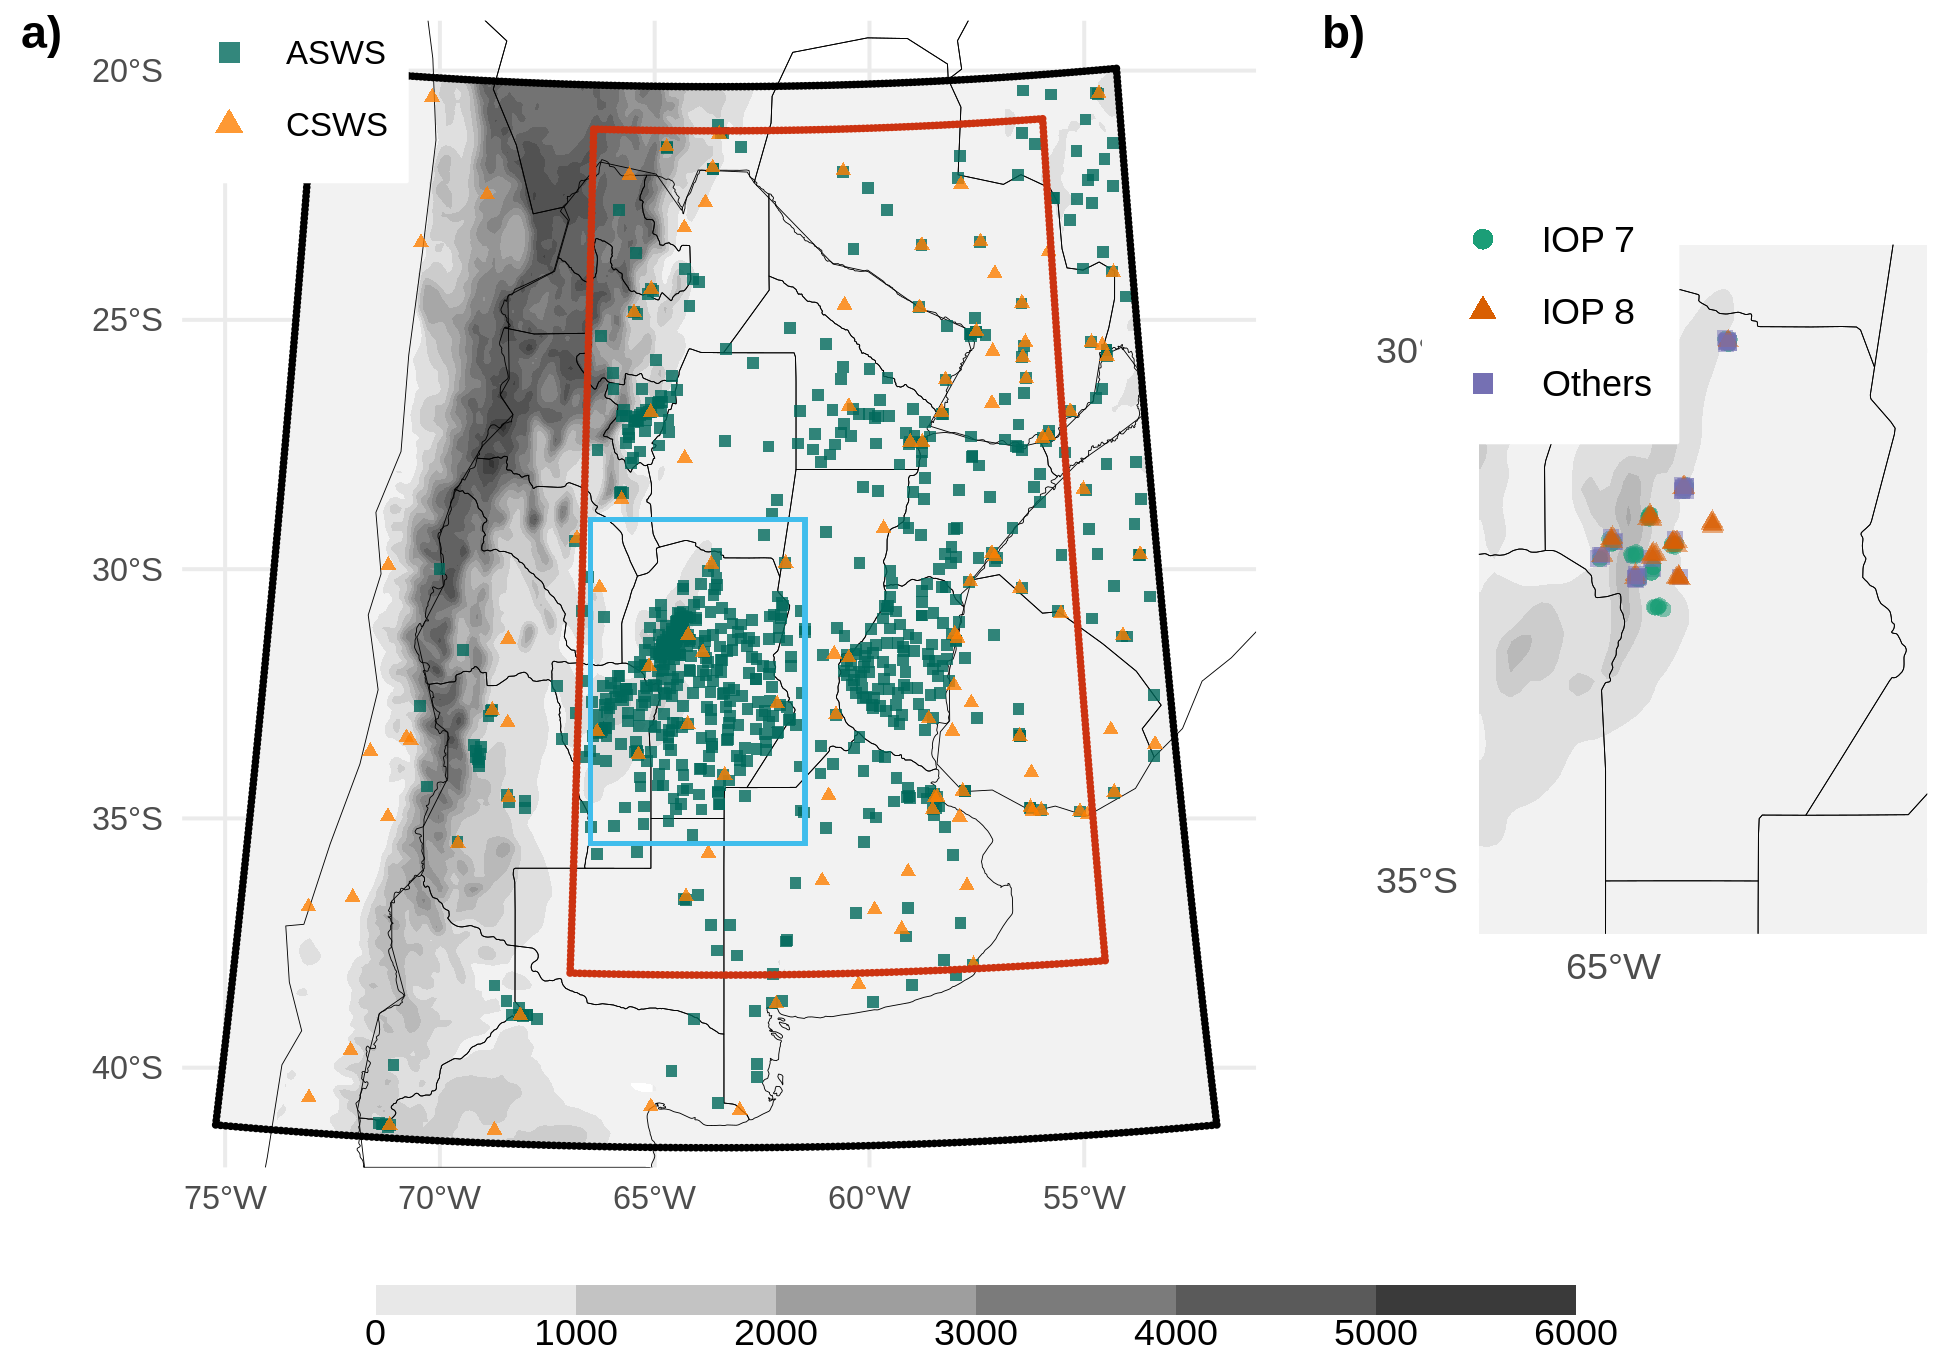
\includegraphics[width=1\linewidth]{../figures/dominio-1} \caption{a) The domain used for the simulations (black box), the inner domain used for the experiment comparison (red box), the region shown in b) (light blue box), and the locations of Automatic Weather Stations (AWS, green squares) and Conventional Surface Weather Stations (CSWS, orange triangles). b) Locations of radiosonde launches during the RELAMPAGO. Green dots correspond to radiosondes launched during IOP 7, orange triangles are radiosondes launched during IOP 8, and purple squares are radiosondes launched outside the IOP missions. The topography in meters is also shown (shaded).}\label{fig:dominio}
\end{figure}

\hypertarget{observations}{%
\subsection{Observations}\label{observations}}

\hypertarget{conventional}{%
\subsubsection{Conventional}\label{conventional}}

The conventional observations used are part of the Global Data Assimilation System (GDAS) data stream. We assimilated conventional observations included in the Binary Universal Form for Representation of Meteorological Data (PREPBUFR) files generated at the National Centers for Environmental Prediction (NCEP). These consist of surface observations from 117 Conventional Surface Weather Stations (CSWS), ships, and upper-air observations from 13 radiosondes sites and aircraft. The orange triangles in Figure \ref{fig:dominio} indicate the location of the surface stations included in this experiment. The frequency of these observations varied between 1 hour for surface stations and 12/24 hours for radiosondes. Wind surface observations over oceans (ASCATW) come from scatterometers and are also included in the PREPBUFR files.

Table \ref{tab:table-obs} lists all the observation types (i.e., surface pressure, temperature, specific humidity, and wind) available for each source, together with their associated errors. The observation errors were specified following the GSI default configuration. In some cases, the error varies with height and depends on the specific platform (aircraft and satellite-derived wind). In terms of quality control, a gross check was performed by the observation operator by comparing the innovation (the difference between the observation and the model-simulated observation based on the first-guess) with a predefined threshold that depends on the observation error (also included in Table \ref{tab:table-obs}).

\hypertarget{aws-networks}{%
\subsubsection{AWS networks}\label{aws-networks}}

We also assimilate data from 866 Automatic Weather Stations (AWS) that are part of 17 public and private surface networks over Southern South America. The dataset used in this study has been obtained from the RELAMPAGO Data Set repository (Garcia et al., 2019). These stations are indicated as green squares in Figure \ref{fig:dominio}a. They have higher spatial coverage than the CSWS and a sampling frequency of 10 minutes in most cases. All stations measure temperature, but only 395 stations provide humidity, 422 provide pressure, and 605 provide wind information.
Observation errors used to assimilate these observations are the same as for the CSWS (see Table \ref{tab:table-obs}).

\hypertarget{satellite-derived-winds}{%
\subsubsection{Satellite derived winds}\label{satellite-derived-winds}}

Satellite-derived wind observations are also included in the PREPBUFR files available every 6 h, and consist of estimations from GOES-16 (using the visible, infrared, and water vapor channels) and METEOSAT 8 and 11 (using the visible and water vapor channels). Due to the domain covered by each of these satellites, GOES-16 is the primary source of satellite-derived winds (99 \% of the observations). Observation errors used to assimilate these observations are indicated in Table \ref{tab:table-obs}.

\begin{table}

\caption{\label{tab:table-obs}Characteristics of the assimilated observations: The code for each observation type and its source, the available variables, the observation error, and the gross check thresholds used.}
\centering
\fontsize{6}{8}\selectfont
\begin{tabular}[t]{>{\raggedright\arraybackslash}p{3.5em}>{\raggedright\arraybackslash}p{4.5em}>{\raggedright\arraybackslash}p{5em}>{\raggedright\arraybackslash}p{7em}>{\raggedright\arraybackslash}p{7em}}
\toprule
Code & Platform & Variable & Error & Gross check\\
\midrule
 &  & Pressure & 1-1.6 $hPa^*$ & 3.6 $hPa$\\

 &  & Temperature & 1.5 $K$ & 7 $K$\\

 &  & Specific humidity & 20 \% & 8 $gKg^{-1}$\\

\multirow{-4}{3.5em}{\raggedright\arraybackslash CSWS   AWS} & \multirow{-4}{4.5em}{\raggedright\arraybackslash Surface weather stations} & Wind & 2.2 $ms^{-1}$ & 6 $ms^{-1}$\\
\cmidrule{1-5}
 &  & Pressure & 1.1-1.2 $hPa^{**}$ & 4 $hPa$\\

 &  & Temperature & 0.8-1.5 $K^*$ & 8 $K$\\

 &  & Specific humidity & 20 \% & 8 $gKg^{-1}$\\

\multirow{-4}{3.5em}{\raggedright\arraybackslash ADPUPA} & \multirow{-4}{4.5em}{\raggedright\arraybackslash Radiosondes} & Wind & 1.4-3 $ms^{-1}$* & 8 $ms^{-1}$\\
\cmidrule{1-5}
 &  & Temperature & 1.47-2.5 $K^+$ & 7 $K$\\

\multirow{-2}{3.5em}{\raggedright\arraybackslash AIRCFT} & \multirow{-2}{4.5em}{\raggedright\arraybackslash Aircrafts} & Wind & 2.4-3.6 $ms^{-1+}$ & 6.5-7.5 $ms^{-1+}$\\
\cmidrule{1-5}
ASCATW & Advanced Scatterometers & Wind & 1.5 $ms^{-1}$ & 5 $ms^{-1}$\\
\cmidrule{1-5}
 &  & Pressure & 1.3 $hPa$ & 4 $hPa$\\

 &  & Temperature & 2.5 $K$ & 7 $K$\\

 &  & Specific humidity & 20 \% & 8 $gKg^{-1}$\\

\multirow{-4}{3.5em}{\raggedright\arraybackslash SFCSHP} & \multirow{-4}{4.5em}{\raggedright\arraybackslash Ships and Buoys} & Wind & 2.5 $ms^{-1}$ & 5 $ms^{-1}$\\
\cmidrule{1-5}
SATWND & Satellite-derived winds & Wind & 3.8-8 $ms^{-1*+}$ & 1.3-2.5 $ms^{-1+}$\\
\bottomrule
\multicolumn{5}{l}{\rule{0pt}{1em}\textsuperscript{*} Observation error varied with height.}\\
\multicolumn{5}{l}{\rule{0pt}{1em}\textsuperscript{**} Observations above 600 hPa are rejected.}\\
\multicolumn{5}{l}{\rule{0pt}{1em}\textsuperscript{+} Observation error depends on the report type.}\\
\end{tabular}
\end{table}

\hypertarget{sat}{%
\subsubsection{Satellite radiances}\label{sat}}

Satellite radiances available through the GDAS data stream, consisting of infrared and microwave observations, are used in this study. This includes the Advanced Microwave Sounding Unit - A (AMSU-A), Microwave Humidity Sounder (MHS), and 2 multispectral sensors; the Atmospheric Infrared Sounder (AIRS) and the Infrared Atmospheric Sounding Interferometer (IASI) over several satellite platforms (see Table 2). Since the regional domain is located in the mid-latitudes and the satellite platforms of interest are on polar orbits, each sensor scans the area only twice a day with a spatial coverage depending on the satellite swath. For this reason, the number of satellite observations varied significantly among cycles. In particular, the multispectral sensors provided between 100 and 1000 observations for every scan every 12 hours, contributing 88 \% of the total amount of assimilated radiances in our experiment. The vertical location of each radiance observation was estimated as the model level at which its weighting function was maximized as calculated by CRTM. The multispectral sensors have good vertical coverage and are able to sense from the lower troposphere up to the lower stratosphere.
The channels accepted for assimilation and their associated errors were defined taking into account the low model top (50 hPa). The data preprocessing, which is an essential step in the assimilation of radiances, was performed within the GSI system for each sensor specifically. First, a spatial data thinning is applied using a 60 km grid following (Jones et al., 2013; Lin et al., 2017; Singh et al., 2016), where the observations to be assimilated are chosen based on their distance to the model grid points, the observation quality (based on available data quality information), and the number of available channels (from the same pixel and sensor) that passed the quality control. Also, observations over the sea are preferred to those over land or snow (Hu et al., 2018).

The thinned observations were then bias corrected. The bias correction (BC) has an air-mass dependent and an angle-dependent component (Zhu et al., 2014) and it is calculated as a multi-linear function of N predictors \(p_i(x)\), with associated coefficients \(\beta_i\). Then, the bias corrected brightness temperature (\(BT_{bc}\)) can be obtained as:

\[\mathit{BT_{bc}} =\mathit{ BT} + \sum_{i = 0}^{N} \beta_i p_i (x)\]

GSI has a constant offset bias correction term (\(p_0 = 1\)) and the remaining predictors are the cloud liquid water content (CLW), the temperature lapse rate at the pressure of maximum weight, the square of the temperature lapse rate at the pressure of maximum weight, and the emissivity sensitivity. Scan angle-dependent bias is modeled as a 4th-order polynomial (Zhu et al., 2014).

In the GSI system, the \(\beta_i\) coefficients are trained using a variational estimation method which solves for the \(\beta_i\) that provides the best fit between the simulation and the observations. The coefficients were initialized at 18 UTC Nov 18, 2018 with the GFS system coefficients. The assimilation system was configured to use a constant background error variance of 0.01 to avoid large adjustments in the estimated coefficients at each time.

In our experiments, only clear-sky observations are used. For microwave radiances, observations potentially contaminated by clouds are detected using the scattering and Liquid Water Path (LWP) indexes (Weston et al., 2019; Zhu et al., 2016). For the infrared channels, cloud contaminated observations are detected using the transmittance profile calculated within the CRTM algorithms. Additionally, the GSI quality control for infrared sensors looks for observations over water with a large zenith angle (over 60°) to reject channels near the visible range that can be contaminated with reflection. It also performs an emissivity check for observations over land for both infrared and microwave radiances.

\begin{table}

\caption{\label{tab:table-rad}List of the available sensors over several platforms, the number of accepted channels for the assimilation, and the percentage of assimilated observations calculated over all radiance observations and all cycles.}
\centering
\fontsize{7}{9}\selectfont
\begin{tabu} to \linewidth {>{\raggedright}X>{\raggedright}X>{\raggedleft}X>{\raggedright}X}
\toprule
Sensor & Platform & \makecell[r]{Assimilated\\channels} & \makecell[l]{Percentage\\over total}\\
\midrule
AIRS & AQUA & 52 & 31.63 \%\\
\cmidrule{1-4}
 & NOAA15 & 2 & 3.31 \%\\
\cmidrule{2-4}
 & NOAA18 & 2 & 4.45 \%\\
\cmidrule{2-4}
\multirow[t]{-3}{*}{\raggedright\arraybackslash AMSUA} & METOP-A & 2 & 2.08 \%\\
\cmidrule{1-4}
 & METOP-A & 66 & 52.72 \%\\
\cmidrule{2-4}
\multirow[t]{-2}{*}{\raggedright\arraybackslash IASI} & METOP-B & 68 & 3.47 \%\\
\cmidrule{1-4}
 & NOAA19 & 2 & 0.68 \%\\
\cmidrule{2-4}
 & METOP-A & 3 & 0.8 \%\\
\cmidrule{2-4}
\multirow[t]{-3}{*}{\raggedright\arraybackslash MHS} & METOP-B & 3 & 0.85 \%\\
\bottomrule
\end{tabu}
\end{table}



\begin{figure}
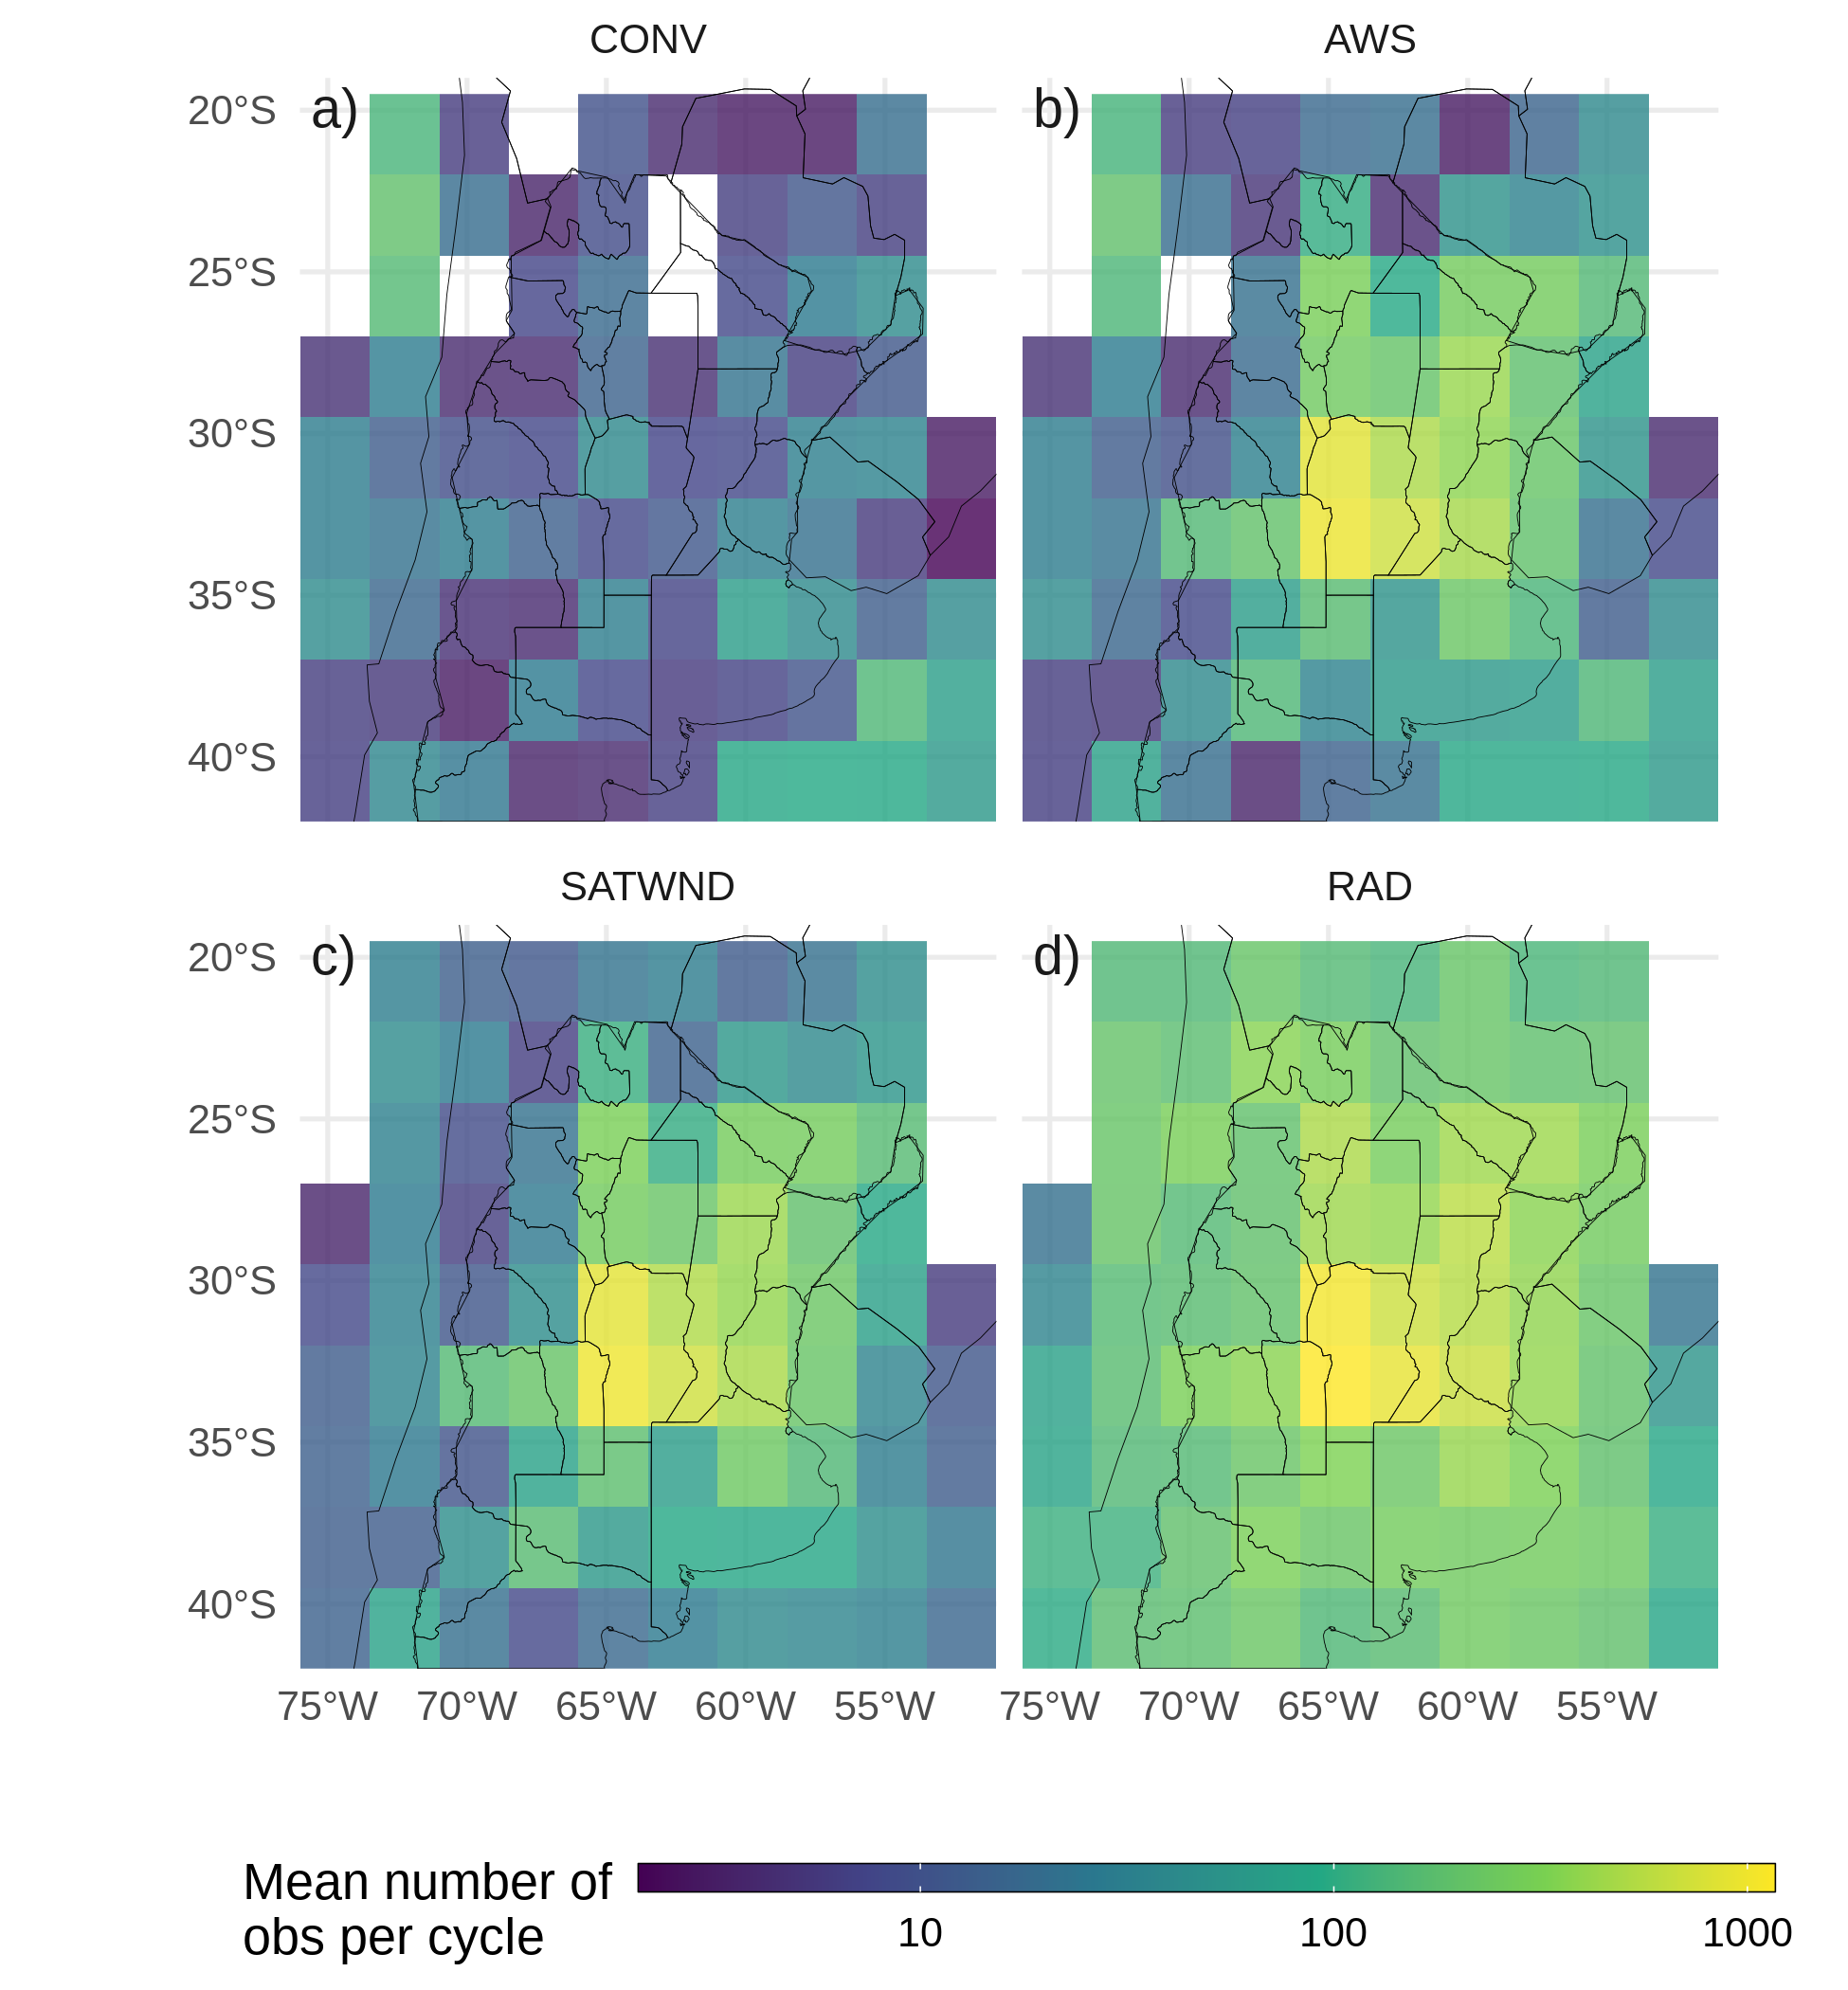
\includegraphics[width=1\linewidth]{../figures/obs-horizontal-1} \caption{Horizontal spatial distribution of the mean available observations per analysis cycle for the a) CONV, b) AWS, c) SATWND, and d) RAD experiments calculated over 2.5\(^{\circ}\) boxes.}\label{fig:obs-horizontal}
\end{figure}



\begin{figure*}
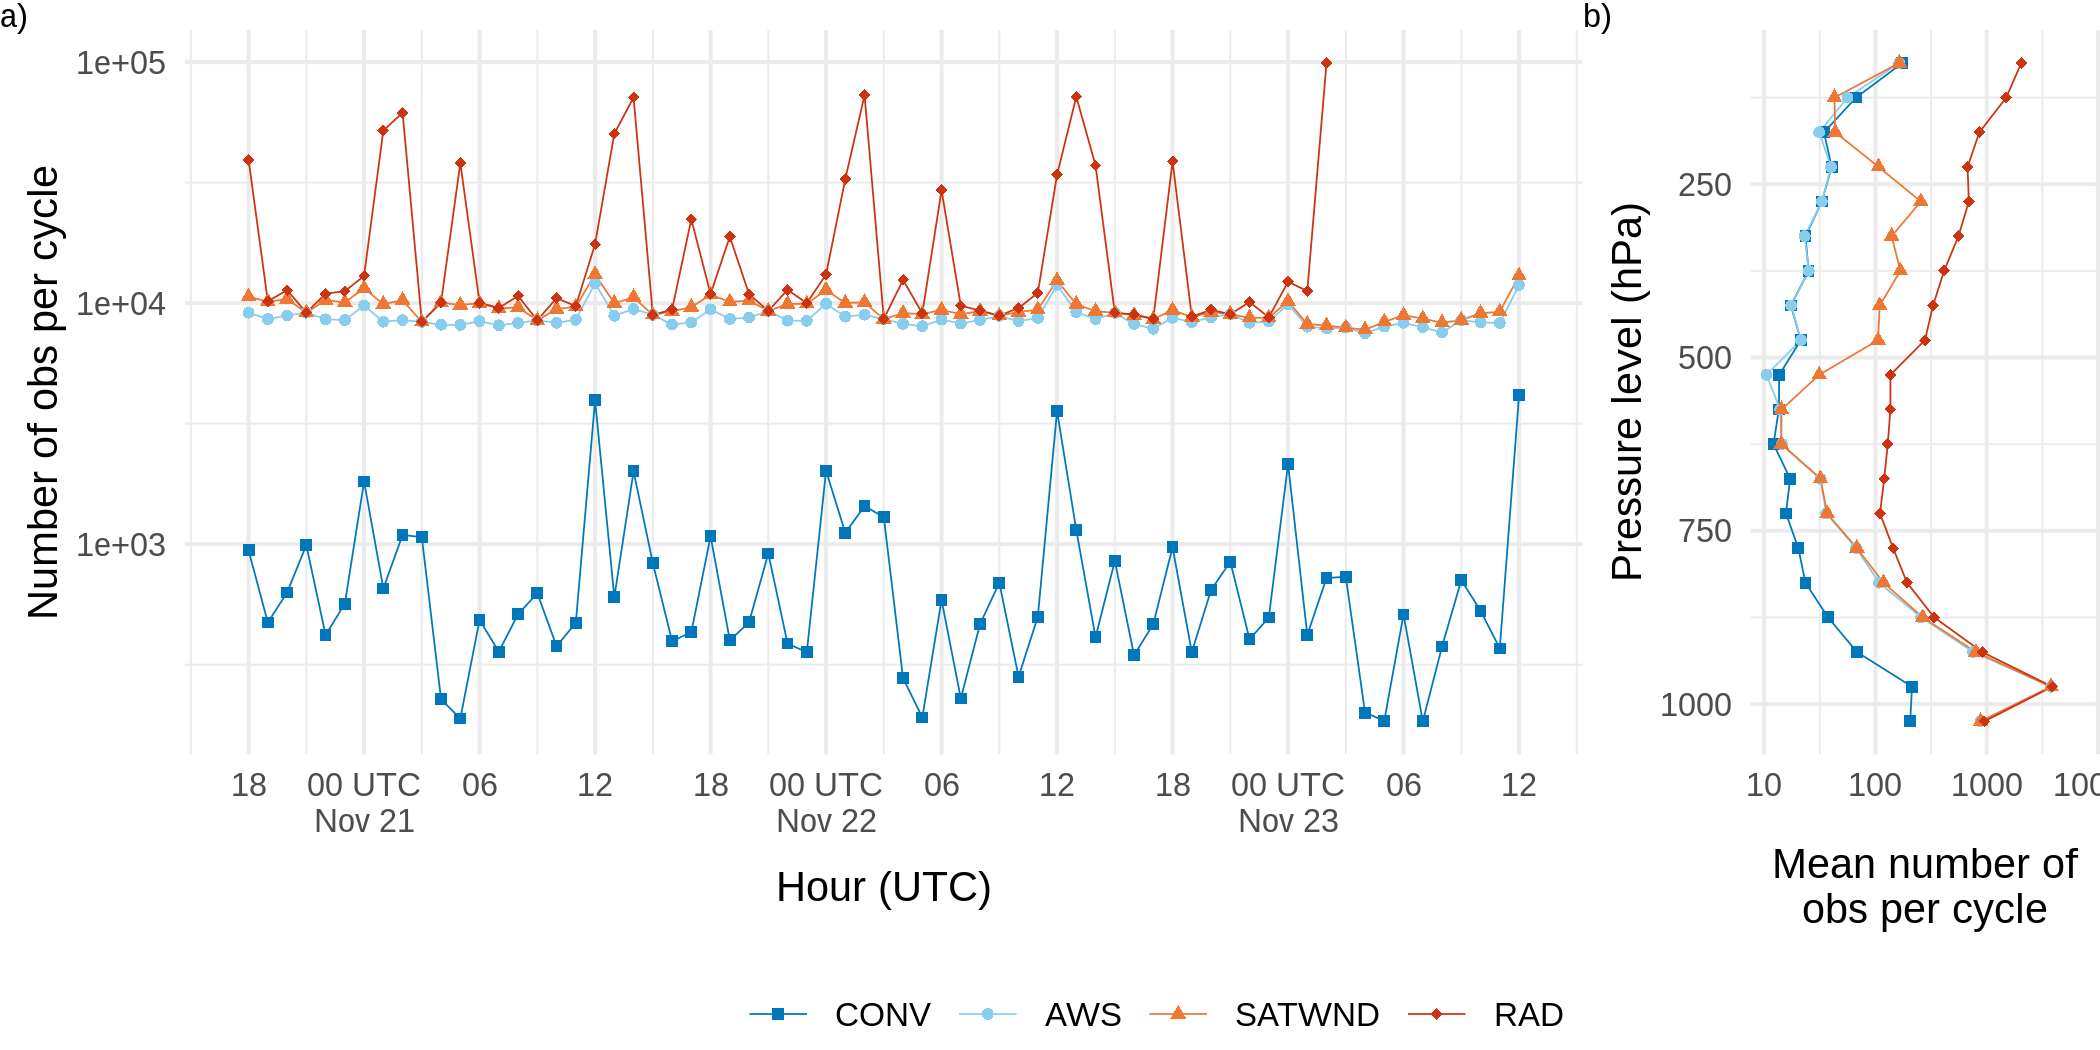
\includegraphics{../figures/obs-cycle-1} \caption{a) Number of assimilated observations per cycle and b) time averaged number of assimilated observations per cycle divided into 50 hPa-depth vertical layers for the CONV (blue squares and line), AWS (light blue dots and line), SATWND (orange triangles and line) and RAD (red diamonds and line) experiments.}\label{fig:obs-cycle}
\end{figure*}

\hypertarget{validation-dataset}{%
\subsubsection{Validation dataset}\label{validation-dataset}}

To evaluate the performance of the ensemble-based DA system presented in this article, we use the following observational datasets:

\begin{itemize}
\item
  The Multi-Network Composite Highest Resolution Radiosonde Data (Earth Observing Laboratory, 2020) from the RELAMPAGO field campaign database consisting of high-resolution radiosondes launched from several locations during the IOPs along with the operational radiosondes. Only the soundings that did not enter the assimilation system were used for validation. The experiment period covers IOP missions 7 and 8, during which 74 radiosondes were launched in a small area near the center of the experimental domain (Figure \ref{fig:dominio}b).
\item
  The Satellite precipitation estimation IMERG Final Run with 0.01\(^{\circ}\) spatial resolution and 30 minutes temporal resolution (Huffman et al., 2018) was used as a reference state to validate the skill of 1-hour forecasts to represent the precipitation over the domain.
\item
  Radar observations are used to perform a qualitative and visual assessment of the convection features. The data comes from 9 radars located in the domain and is provided by the Argentine C-band Doppler dual-polarization weather radar network (de Elía et al., 2017) with a temporal frequency of 10 minutes. For this work, only the maximum reflectivity in the column (COLMAX) closest to the analysis time was used.
\end{itemize}

\hypertarget{exp}{%
\subsection{Experimental design}\label{exp}}

To investigate the impact of different observations upon the analysis, four DA experiments were performed using different observation sets (Table \ref{tab:table-exp}). The CONV experiment uses only conventional observations from PREPBUFR. In a second experiment, referred to as AWS, we assimilate all the observations included in CONV plus the 10-minute frequency surface observations from AWS. In the third experiment, referred to as SATWND, we assimilate all the observations of the AWS experiment and the satellite-derived winds. Finally, a fourth experiment referred to as RAD assimilates all available clear-sky radiances from sensors onboard polar orbiting satellites as described in section \ref{sat}.

The horizontal distribution of the average number of assimilated observations per cycle in each experiment is shown in Figure \ref{fig:obs-horizontal}. The larger number of assimilated observations over the center and east of the domain corresponds to the AWS observations. In Figure \ref{fig:obs-cycle}a the number of assimilated observations over time is shown. Local maxima at 12 and 00 UTC found mainly in CONV are attributed to operational soundings. The strong variability in the number of radiance observations per cycle is also noticeable and depends on the satellite coverage. The maxima at 13-14 and 01-02 UTC in RAD correspond to the contribution of the multispectral sensors. The vertical distribution of the mean number of observations per cycle (Figure \ref{fig:obs-cycle}b) shows a maximum in low levels due to the AWS observations. Satellite-derived winds are maximized at the upper troposphere (between 500-250 hPa). Above 850 hPa, most of the observations correspond to radiance observations.

All the assimilation experiments start at 18 UTC Nov 20, 2018 and continue until 12 UTC Nov, 23 (totaling 67 hours/assimilation cycles). The initial 60-member ensemble is generated as explained in section \ref{config} from a spin-up run without assimilating observations performed between 12 UTC and 18 UTC Nov, 20 (Figure \ref{fig:cycle}).

Ensemble forecasts initialized from the different analysis experiments at 00 and 06 UTC Nov 22 were performed to evaluate the impact of the different observing networks on short range precipitation forecasts. Both forecasts are integrated until 12 UTC Nov 23. All forecasts use the same domain and ensemble configuration as the analysis. The boundary conditions for the ensemble members are generated by adding random perturbations to the GFS deterministic forecast (0.25\(^{\circ}\) horizontal grid spacing and 6-hour temporal resolution; National Centers for Environmental Prediction, National Weather Service, NOAA, U.S. Department of Commerce (2015)).

\begin{table}

\caption{\label{tab:table-exp}Observation types assimilated in each experiment.}
\centering
\begin{tabu} to \linewidth {>{\raggedright\arraybackslash}p{8em}>{\centering\arraybackslash}m{2.5em}>{\centering\arraybackslash}m{2.5em}>{\centering\arraybackslash}m{3em}>{\centering\arraybackslash}m{3em}}
\toprule
Obs type & CONV & AWS & SATWND & RAD\\
\midrule
Conventional (PREPBUFR) & x & x & x & x\\
Conventional (AWS) &  & x & x & x\\
Satellite-derived winds &  &  & x & x\\
Radiances &  &  &  & x\\
\bottomrule
\end{tabu}
\end{table}



\begin{figure}
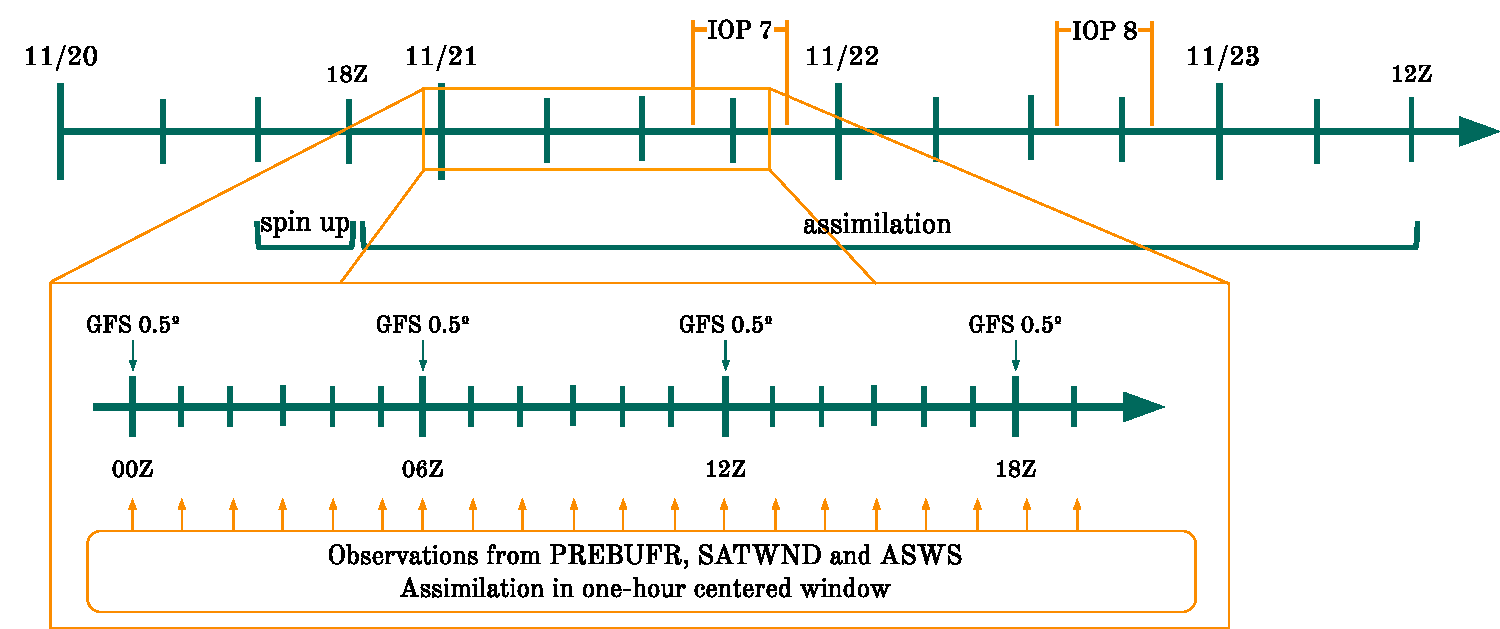
\includegraphics[width=1\linewidth]{/home/paola.corrales/mesoda/analysis/figures/analysis_cycle} \caption{Figure 4. Diagram of the analysis cycles between 18 UTC Nov 20, and 12 UTC Nov 23 plus spin up period of 6 hours. The zoomed section shows the hourly assimilation that is performed within a one-hour centered window and new boundary conditions from GFS every 6 hours. The two IOP missions from the RELAMPAGO field campaign and the ensemble forecast initialized at 00 and 06 UTC Nov 22 are shown.}\label{fig:cycle}
\end{figure}

\hypertarget{verification-methods}{%
\subsection{Verification methods}\label{verification-methods}}

A set of metrics are selected to evaluate different aspects of the analysis obtained in the experiments conducted in this paper. These aspects include a validation of how the uncertainty is quantified in the first-guess and in the analysis, and how different experiments fit an independent set of observations that are not assimilated.

To evaluate the consistency of the uncertainty quantification in the first-guess and in the analysis we use the Reduced Centered Random Variable (RCRV, Candille et al. (2007)) which is defined as:

\[RCRV = \frac{x_o - m}{\sqrt{\sigma_o^2 + \sigma^2}}\]

where \(x_o\) is the assimilated observation and its error \(\sigma_o\), the ensemble mean of the analysis in observational space \(m\), and the standard deviation \(\sigma\) of the ensemble.
The average of \(RCRV\) computed over all the realizations represents the bias of the ensemble mean with respect to the observations normalized by the estimated uncertainty:

\[\mathit{mean RCRV} = E[RCRV]\]

The standard deviation of the \(RCRV\) or \(sd RCRV\) measures the agreement of the ensemble spread and the observational error with respect to the distance between the ensemble mean and the observations, and then the systematic over- or under- dispersion of the ensemble:

\[\mathit{sd RCRV} = \sqrt{\frac{M}{M -1}E[(\mathit{RCRV} - \mathit{mean RCRV})^2]}\]

where \(M\) is the ensemble size. A consistent system will have no bias (\(mean RCRV = 0\)) and a standard deviation equal to 1 (\(sd RCRV = 1\)). If the ensemble has a positive bias, \(mean RCRV\) will be positive, on the opposite, if the ensemble has a negative bias, \(mean RCRV\) will be negative. A \(sd RCRV > 1\) () indicates that the ensemble is underdispersive and an \(sd RCRV < 1\) indicates that the ensemble is overdispersive.

The fit of the first-guess and analysis to a set of independent observations, the high-resolution radiosondes from RELAMPAGO, is computed based on the Root Mean Square Error (RMSE) and the BIAS:

\[\mathit{RMSE} = \sqrt{\frac{1}{N}\sum_{i = 1}^{N} (X_i - O_i)^{2}}\]

\[\mathit{BIAS} = \frac{1}{N}\sum_{i = 1}^{N} (X_i - O_i)\]

where \(O\) and \(X\) stand for independent observations, and the simulations respectively and N is the sample size.

For the comparison of the first-guess precipitation with the IMERG precipitation estimates, we compute a probabilistic Fractions Skill Score (FSS, Roberts (2008)) for different neighborhood length scales and thresholds. Following Maldonado et al. (2021) the definition of the FSS is slightly modified in that the probability of having rain exceeding a particular threshold and over a particular region is computed taking into account all the ensemble members :

\[\mathit{FSS} = 1-\frac{\frac{1}{N}\sum_{i=1}^{N} ({P_x}_i-{P_o}_i)^{2}}{\frac{1}{N}\sum_{i=1}^{N} ({P_x}_i)^{2}+\frac{1}{N}\sum_{i=1}^{N} ({P_o}_i)^{2}} \]

where \(P_{xi}\) is the probability of occurrence of accumulated rainfall over a specified threshold computed from the ensemble and \(P_{oi}\) is the proportion of grid points in each sampling area in which the observed accumulated precipitation is over the same threshold. Since the precipitation forecast of all the ensemble members is considered in the computation of \(P_{xi}\), the smoothing effect of the ensemble mean is avoided. The FSS was computed from the accumulated precipitation over 6 hr periods by adding the 1-hr accumulated precipitation forecasts over 6 consecutive assimilation cycles.

\hypertarget{computation-procedures}{%
\subsection{Computation procedures}\label{computation-procedures}}

We performed all the experiments at the National Center for Atmospheric Research (NCAR) supercomputer Cheyenne (Computational and Information Systems Laboratory, 2019). All the analyses in this paper were performed using the R programming language (R Core Team, 2020), using data.table (Dowle and Srinivasan, 2020) and metR (Campitelli, 2020) packages.
All graphics are made using ggplot2 (Wickham, 2009) and the paper was rendered using knitr and rmarkdown (Allaire et al., 2019; Xie, 2015).

\hypertarget{results}{%
\section{Results}\label{results}}

\hypertarget{ensemble-consistency}{%
\subsection{Ensemble consistency}\label{ensemble-consistency}}

To investigate the ability of the first-guess ensemble mean to fit the observations taking into account the uncertainties of the forecast and the observations, we calculated the \(mean RCRV\) and the \(sd RCRV\) for the RAD experiment. As this experiment assimilates all types of observations used in this work, it is possible to analyze the consistency of the ensemble by comparing it with each type of observation. Figure 5 shows the \(sd RCRV\) for surface observations box-averaged to a 2.5° grid. The \(sd RCRV\) for wind observations (Figure \ref{fig:rcrv-sfc}a) is close to 1 suggesting a good agreement between the ensemble spread, the forecast error, and the observation error. For the temperature (Figure \ref{fig:rcrv-sfc}b), the results are similar except that for some areas in the west of the domain the \(sd RCRV\) can be as high as 4.5. In this region, the mean innovation was overly large due to the complex terrain leading to large differences between the model topography and the station height.

Figure \ref{fig:rcrv-profile} shows the mean and standard deviation of the RCRV for the upper-air observations. Figures \ref{fig:rcrv-profile}a-b show the RCRV statistics for soundings (ADPUPA) and aircraft (AIRCAR and AIRCFT). Both ADPUPA and AIRCFT show a generally good agreement between the ensemble spread and the observation error. As sounding observations and their associated errors are known to be reliable, this result indicates that the ensemble has an appropriate spread. AIRCAR presents an irregular profile with \(sd RCRV\) values that suggest that the error for this type of observation is overestimated. ADPUPA and AIRCAR present a \(mean RCRV\) profile near zero at middle and upper levels but ADPUPA observations show a cold bias with respect to the model at low levels, a characteristic already studied in Ruiz et al. (2010) and Dillon et al. (2021).

For satellite-derived winds (Figure \ref{fig:rcrv-profile}c) at low levels, where there are not many observations available, the profiles of \(mean RCRV\) and \(sd RCRV\) show a larger departure from the expected behavior with a negative bias, and a possible overestimation of the observation error. Wind estimations derived from water vapor channels are abundant above 500 hPa where their bias is close to zero. The only exception are the EUMETSAT observations which contribute very little in the region.

The mean RCRV profiles calculated from the radiance observations (Figure \ref{fig:rcrv-profile}d) show almost no bias and the same happens if the \(mean RCRV\) is calculated over each channel of each sensor (not shown). This indicates that the bias correction algorithm works as expected. The \(sd RCRV\) values are less than 1 for all sensors possibly due to an overestimation of the observation errors to reduce the influence of potentially erroneous observations.

Overall, these results indicate that the ensemble spread is consistent with the short-range forecast error and that systematic errors are relatively small for most of the observation types used in this work. Moreover, these results suggest the inflation parameter \(\alpha = 0.9\) is adequate for the system.



\begin{figure}
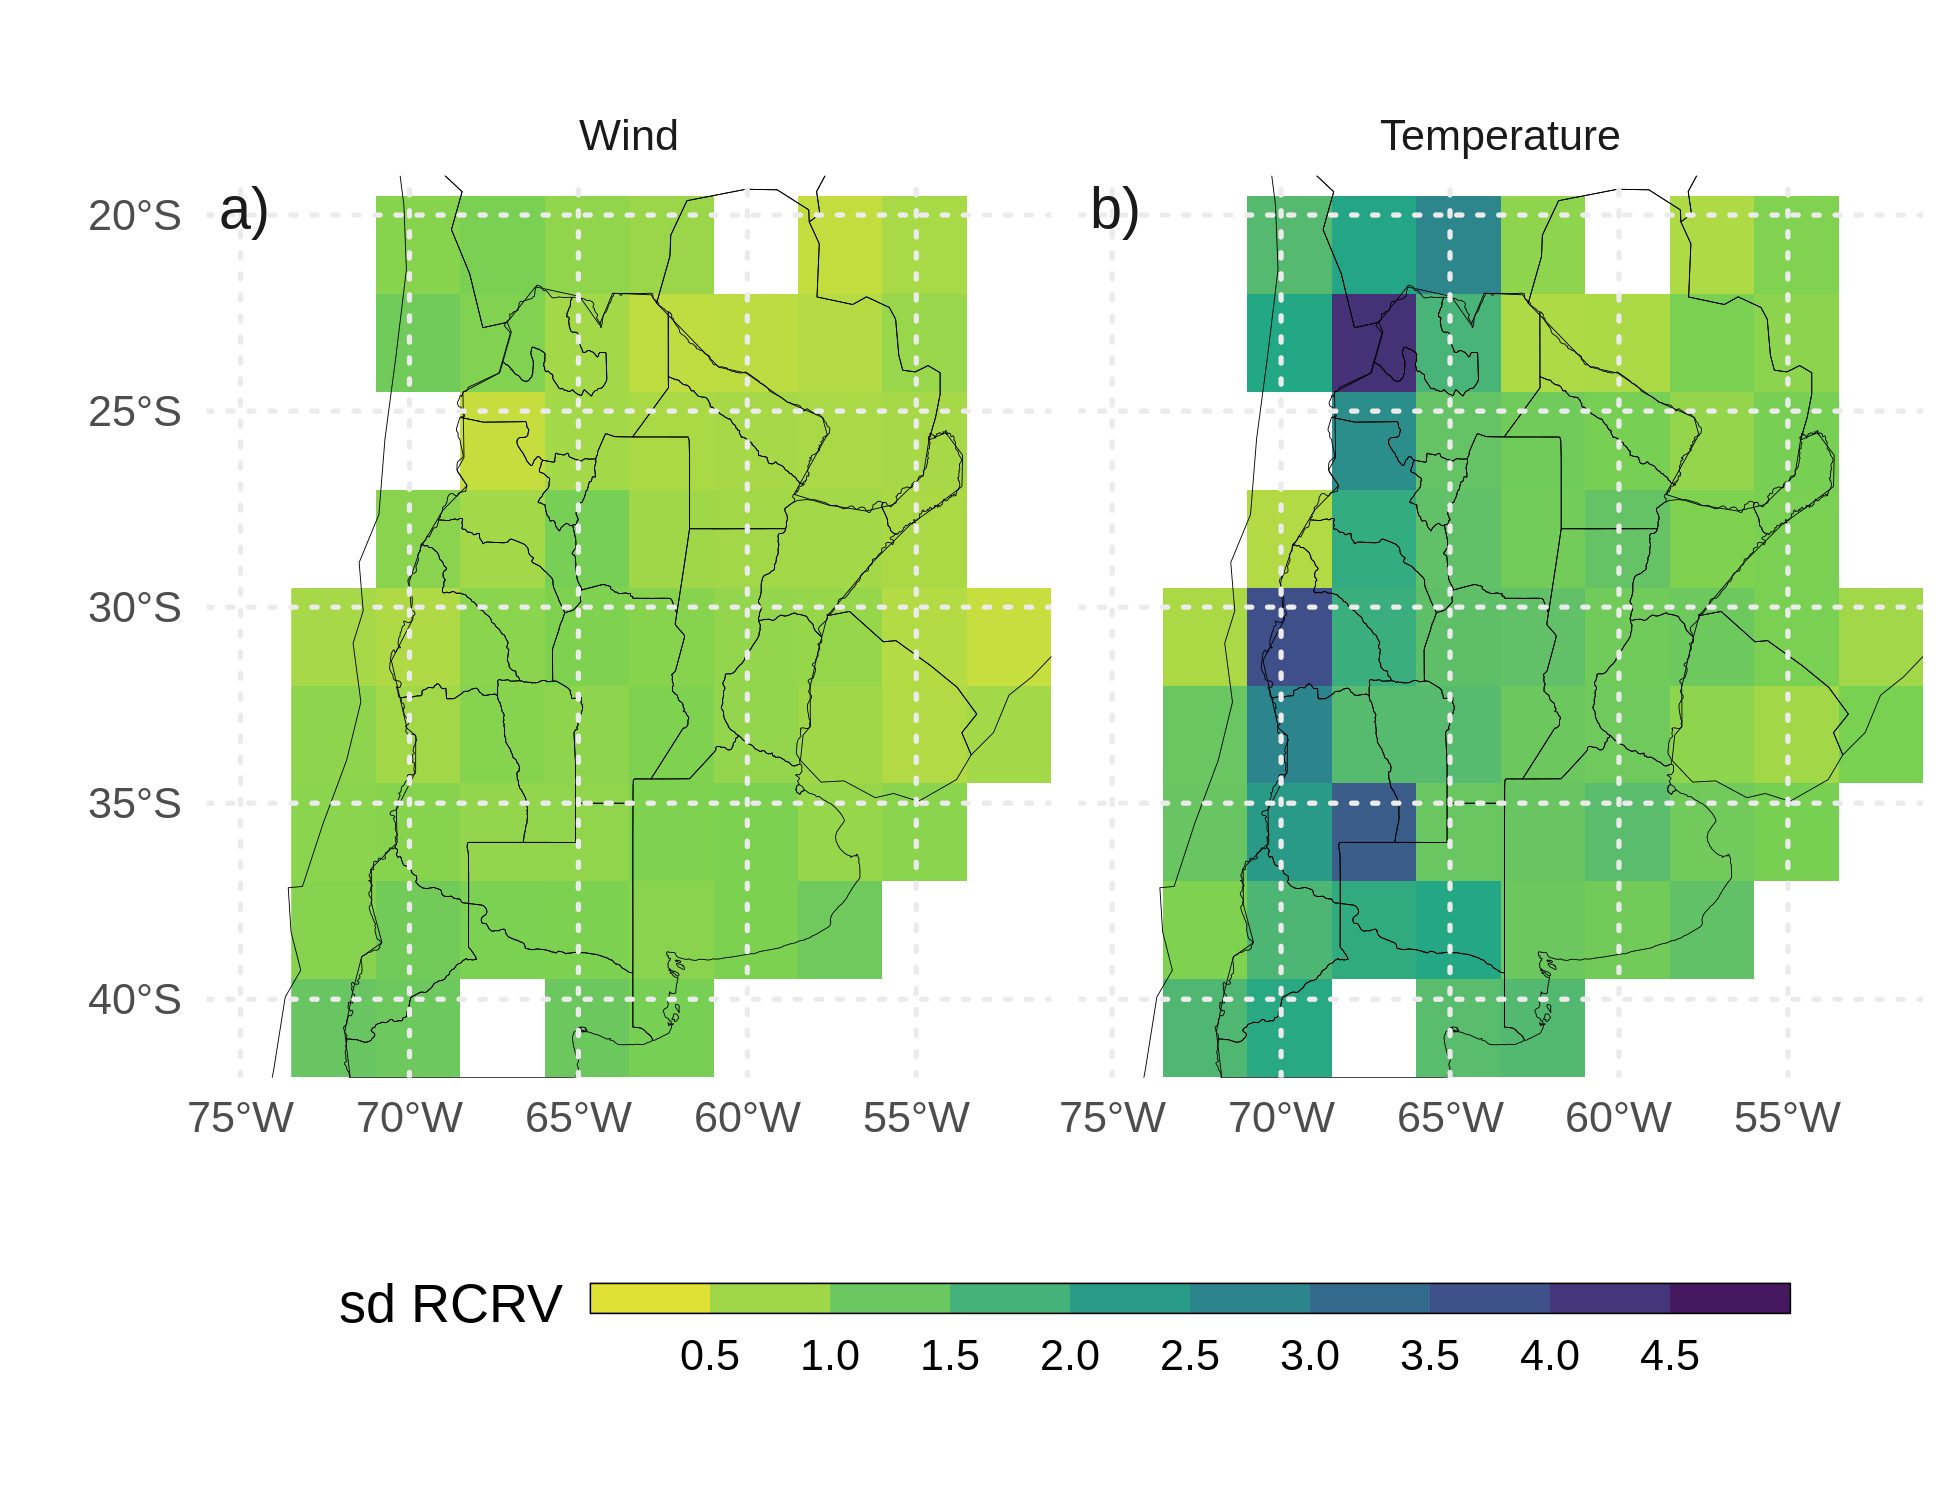
\includegraphics[width=1\linewidth]{../figures/rcrv-sfc-1} \caption{First guess \(sd RCRV\) calculated for surface observations (from PREPBUFR and AWS) of a) wind, and b) temperature averaged over 2.5º boxes for the RAD experiment. Observations were aggregated every hourly cycle for the entire experiment period.}\label{fig:rcrv-sfc}
\end{figure}



\begin{figure*}
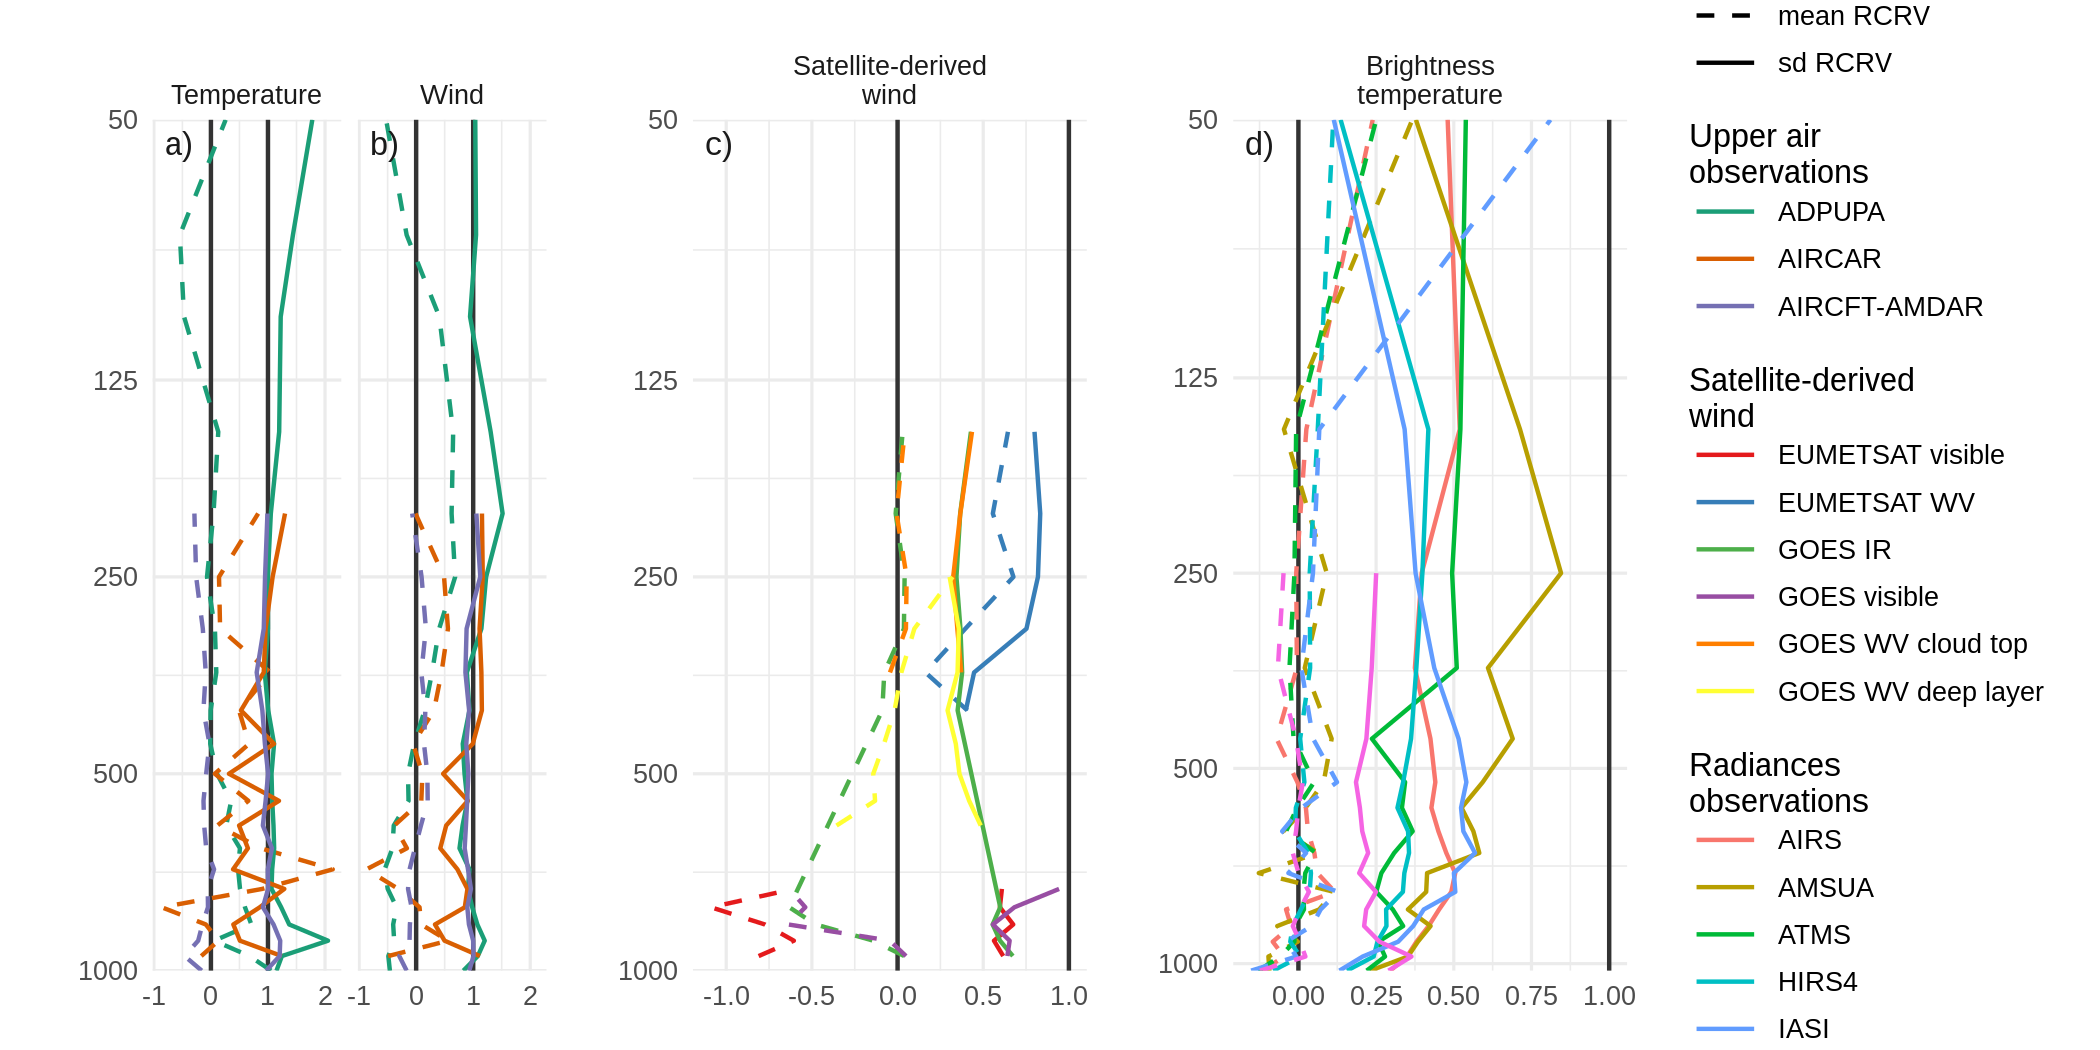
\includegraphics{../figures/rcrv-profile-1} \caption{Vertical profiles of first guess \(mean RCRV\) (dashed line) and \(sd RCRV\) (solid line) for a) temperature and b) wind of sounding and aircraft observations, c) satellite-derived wind observations, and d) brightness temperature observations for the RAD experiment. Observations were aggregated every hourly cycle for the entire experiment period.}\label{fig:rcrv-profile}
\end{figure*}

\hypertarget{impacts-of-assimilated-observations}{%
\subsection{Impacts of assimilated observations}\label{impacts-of-assimilated-observations}}

In this section, we present the impact of assimilating different observation types on variables which are particularly relevant for the occurrence of deep moist convection. The analysis is performed over a smaller domain (red box in Figure \ref{fig:dominio}a) to focus on the region most directly affected by the MCS. Figures \ref{fig:TQ-diff}a-c show the analysis difference between experiments in the spatially averaged vertical profile of temperature. By averaging the differences between two experiments we can isolate the systematic impact produced by different observing systems on the analyzed state. During the first day, the assimilation of AWS observations results in a colder PBL. This cooling effect has a clear diurnal cycle, being stronger during nighttime (Figure \ref{fig:TQ-diff}a). During the second day of the experiment, the impact of AWS observations extends into the middle and upper troposphere coinciding with the mature stage of the MCS. The warm difference shown in AWS-CONV between 500 and 200 hPa is produced by the development of stronger convection in AWS compared to CONV. This is a good example of how low-level information provided by surface weather stations can rapidly spread into the troposphere in the presence of deep moist convection. Although the mid-to-upper circulation can have an important impact on the organization and evolution of the MCS over the region, the satellite-derived winds did not have an appreciable impact on the mean temperature and humidity (Figure \ref{fig:TQ-diff}b-e), possibly due to the large observation errors used for the assimilation.
During the first day of the experiment, the assimilation of radiances produces a warming effect in the PBL which partially compensates for the cooling effect of AWS observations (Figure \ref{fig:TQ-diff}c). No clear systematic impact is found above the PBL during this period. During the second day, the impact of radiance observations is found through the troposphere with a distribution that is similar to the impact found in the AWS experiment but with the opposite sign.

Comparing the specific humidity in the experiments (Figures \ref{fig:TQ-diff}d-f), the impact of assimilating AWS with fine spatial and temporal resolution is most substantial at low levels (Figure \ref{fig:TQ-diff}d). The PBL in the AWS experiment is consistently moister than in the CONV experiment particularly at nighttime. The increase in low-level moisture by a denser surface network is consistent with previously reported dry biases in the WRF model over the region (Ruiz et al., 2010). We found that the moistening of the PBL is mainly driven by the covariance between temperature and specific humidity within the PBL. In our experiment and over the center of the domain, this covariance remains negative, increasing low-level moisture as the observations introduce negative temperature corrections. As for the temperature, the systematic impact of satellite-derived winds on moisture is small (Figure \ref{fig:TQ-diff}e). Figure \ref{fig:TQ-diff}f shows that radiances reduce low-middle level moisture during the first day of the experiment. The drying effect extends to lower-middle levels during the second day of the experiment coinciding with the development of the MCS between 00 and 12 UTC Nov 22.



\begin{figure*}[th]

{\centering 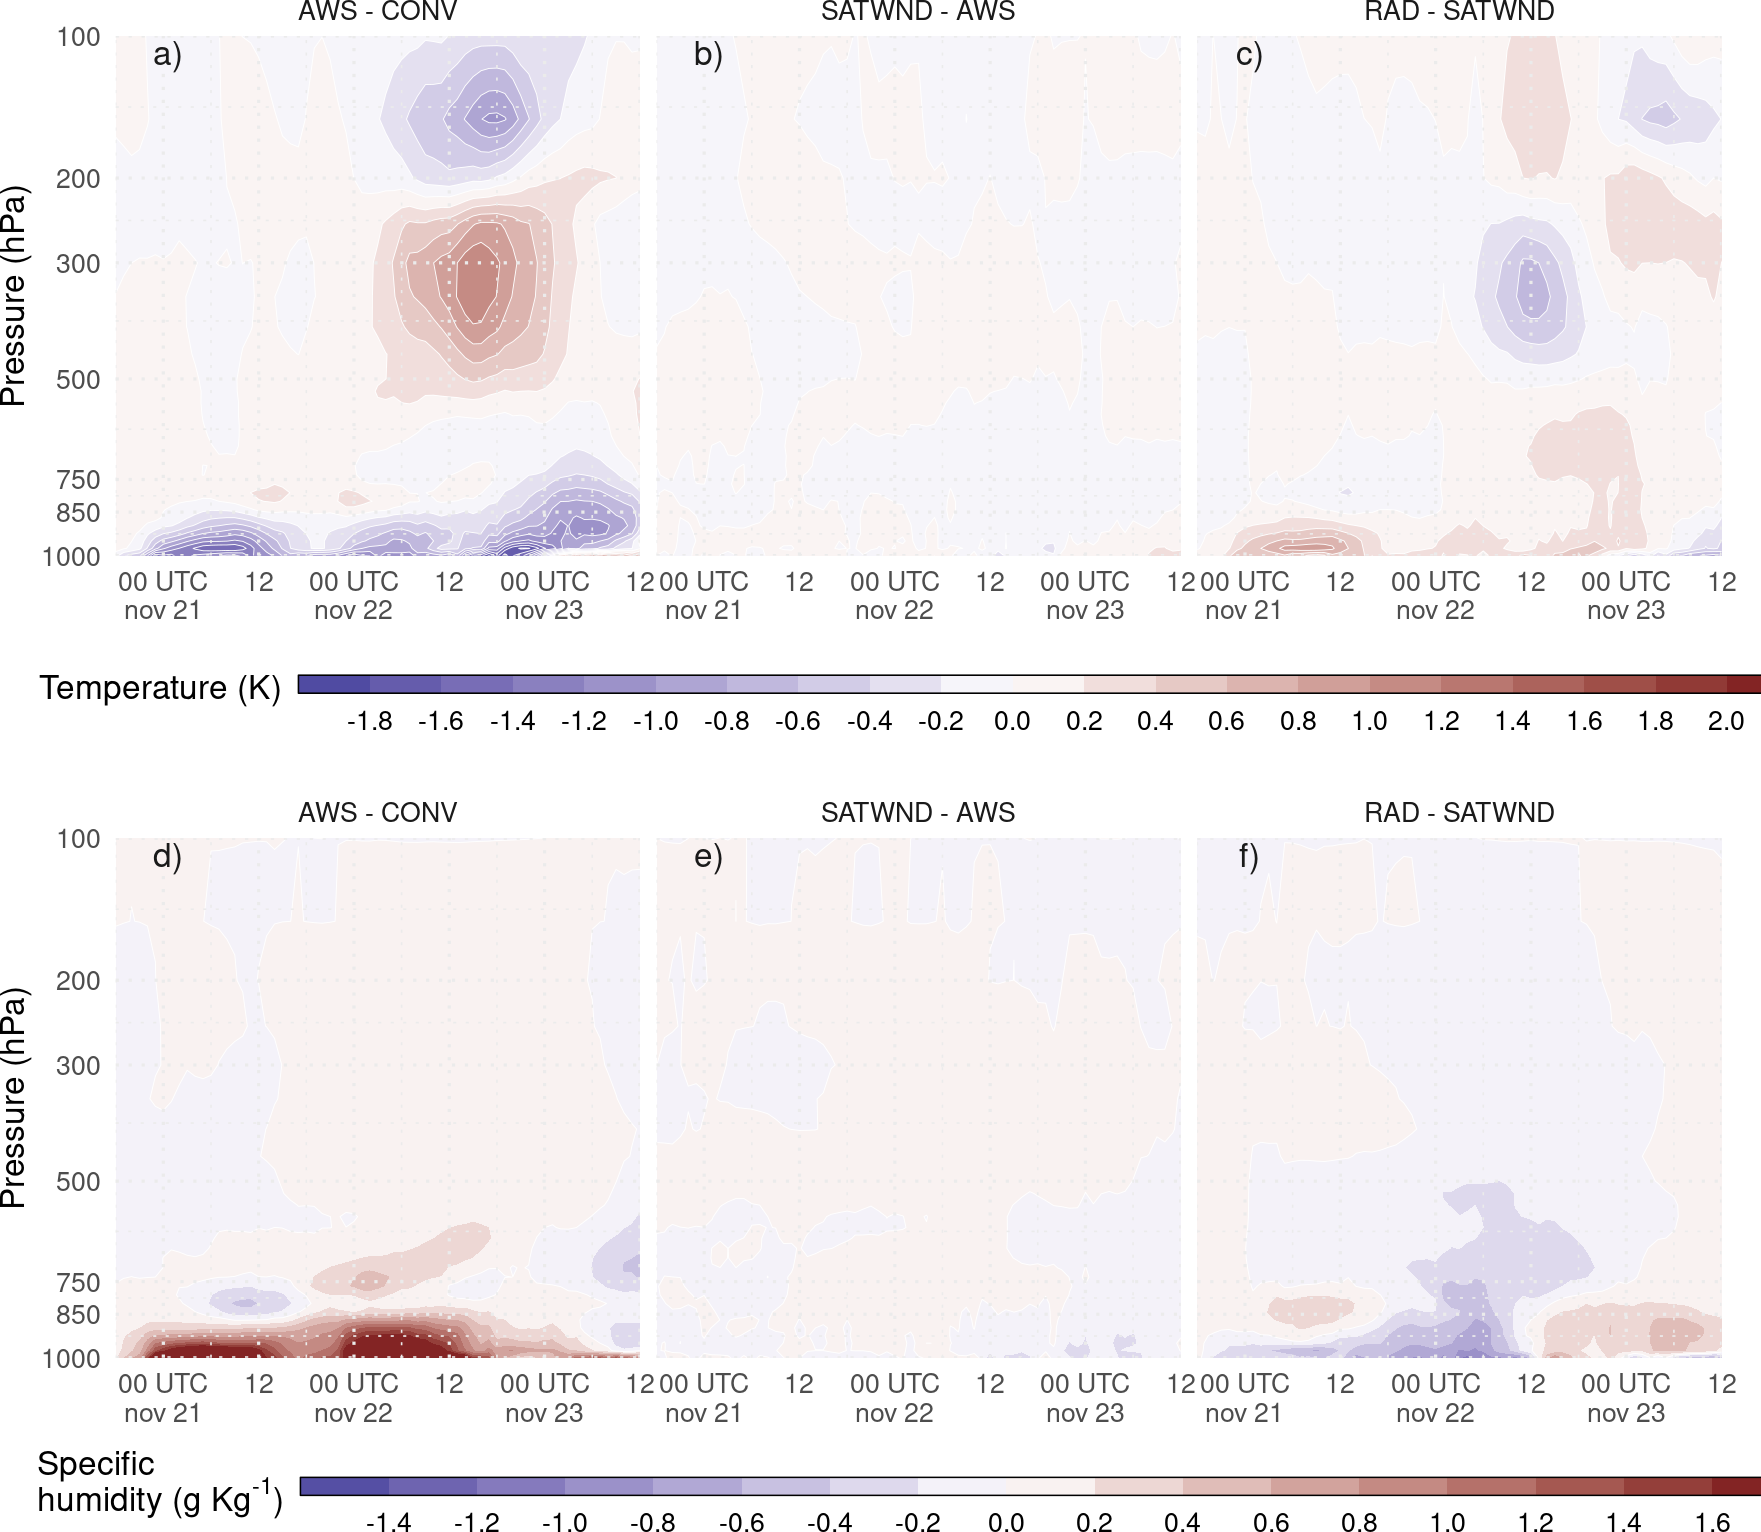
\includegraphics{../figures/TQ-diff-1} 

}

\caption{Difference between analysis ensemble mean experiments a) and d) AWS-CONV, b) and e) SATWND-AWS, and c) and f) RAD-SATWND for the spatially averaged vertical profiles of temperature (a, b, and c, in \(K\)) and specific humidity (d, e, and f in \(gkg^{-1}\)) calculated over the inner domain (red box in Figure \ref{fig:dominio}a) for each analysis cycle.}\label{fig:TQ-diff}
\end{figure*}

The impacts on the wind components are shown in Figure \ref{fig:UV-diff}, along with the corresponding averaged wind component in the experiment with the largest number of assimilated observations (for example, Figure \ref{fig:UV-diff}a shows the zonal wind difference between AWS and CONV and the zonal wind for AWS). The assimilation of AWS produces a more easterly wind and a less northerly wind at low levels during the first two days of analysis (Figures \ref{fig:UV-diff}a,b). There is a diurnal cycle in the impact of surface weather stations on the meridional velocity (Figure \ref{fig:UV-diff}d) with a stronger reduction of the northerly wind during night hours. This indicates that surface observations are reducing the intensity of the low level jet present in the pre-convective environment. After 18 UTC Nov 22, the opposite effect is observed when the MCS is moving through the domain. After the initiation of the convective cells, the systematic impact on the wind field is larger at mid and upper levels (Figures \ref{fig:UV-diff}d, f). During Nov 22 and 23 the impact of assimilating AWS observations produces an increase of northerly wind in upper levels. This could be a consequence of a stronger MCS with an increased polar side upper level outflow. Although satellite-derived wind observations produce the largest impact in mid-to-upper levels where the number of observations is largest; the systematic impact is overall smaller than the one produced by assimilating data from AWS (Figures \ref{fig:UV-diff}b, e).

The assimilation of radiances produces a reduction in the westerly wind compared with respect to SATWIND in low and upper levels (Figure \ref{fig:UV-diff}c). For the meridional wind, these observations produce an enhancement on average of the northerly low-level flow of \(1 ms^{-1}\), opposite to what is generated by the assimilation of AWS observations during the nights, between 03 and 12 UTC, previous to the development of the MCS (Figure \ref{fig:UV-diff}f). At upper levels and during Nov 22 and 23 the average impact of assimilating radiances is a decrease in the wind speed. The meridional wind field at 200 hPa at different times shows that the outflow from the MCS is even more intense than in the other experiments, while the southerly wind ahead of the MCS also increases producing an average reduction of the northerly wind (Figure \ref{fig:UV-diff}f).



\begin{figure*}[ht]

{\centering 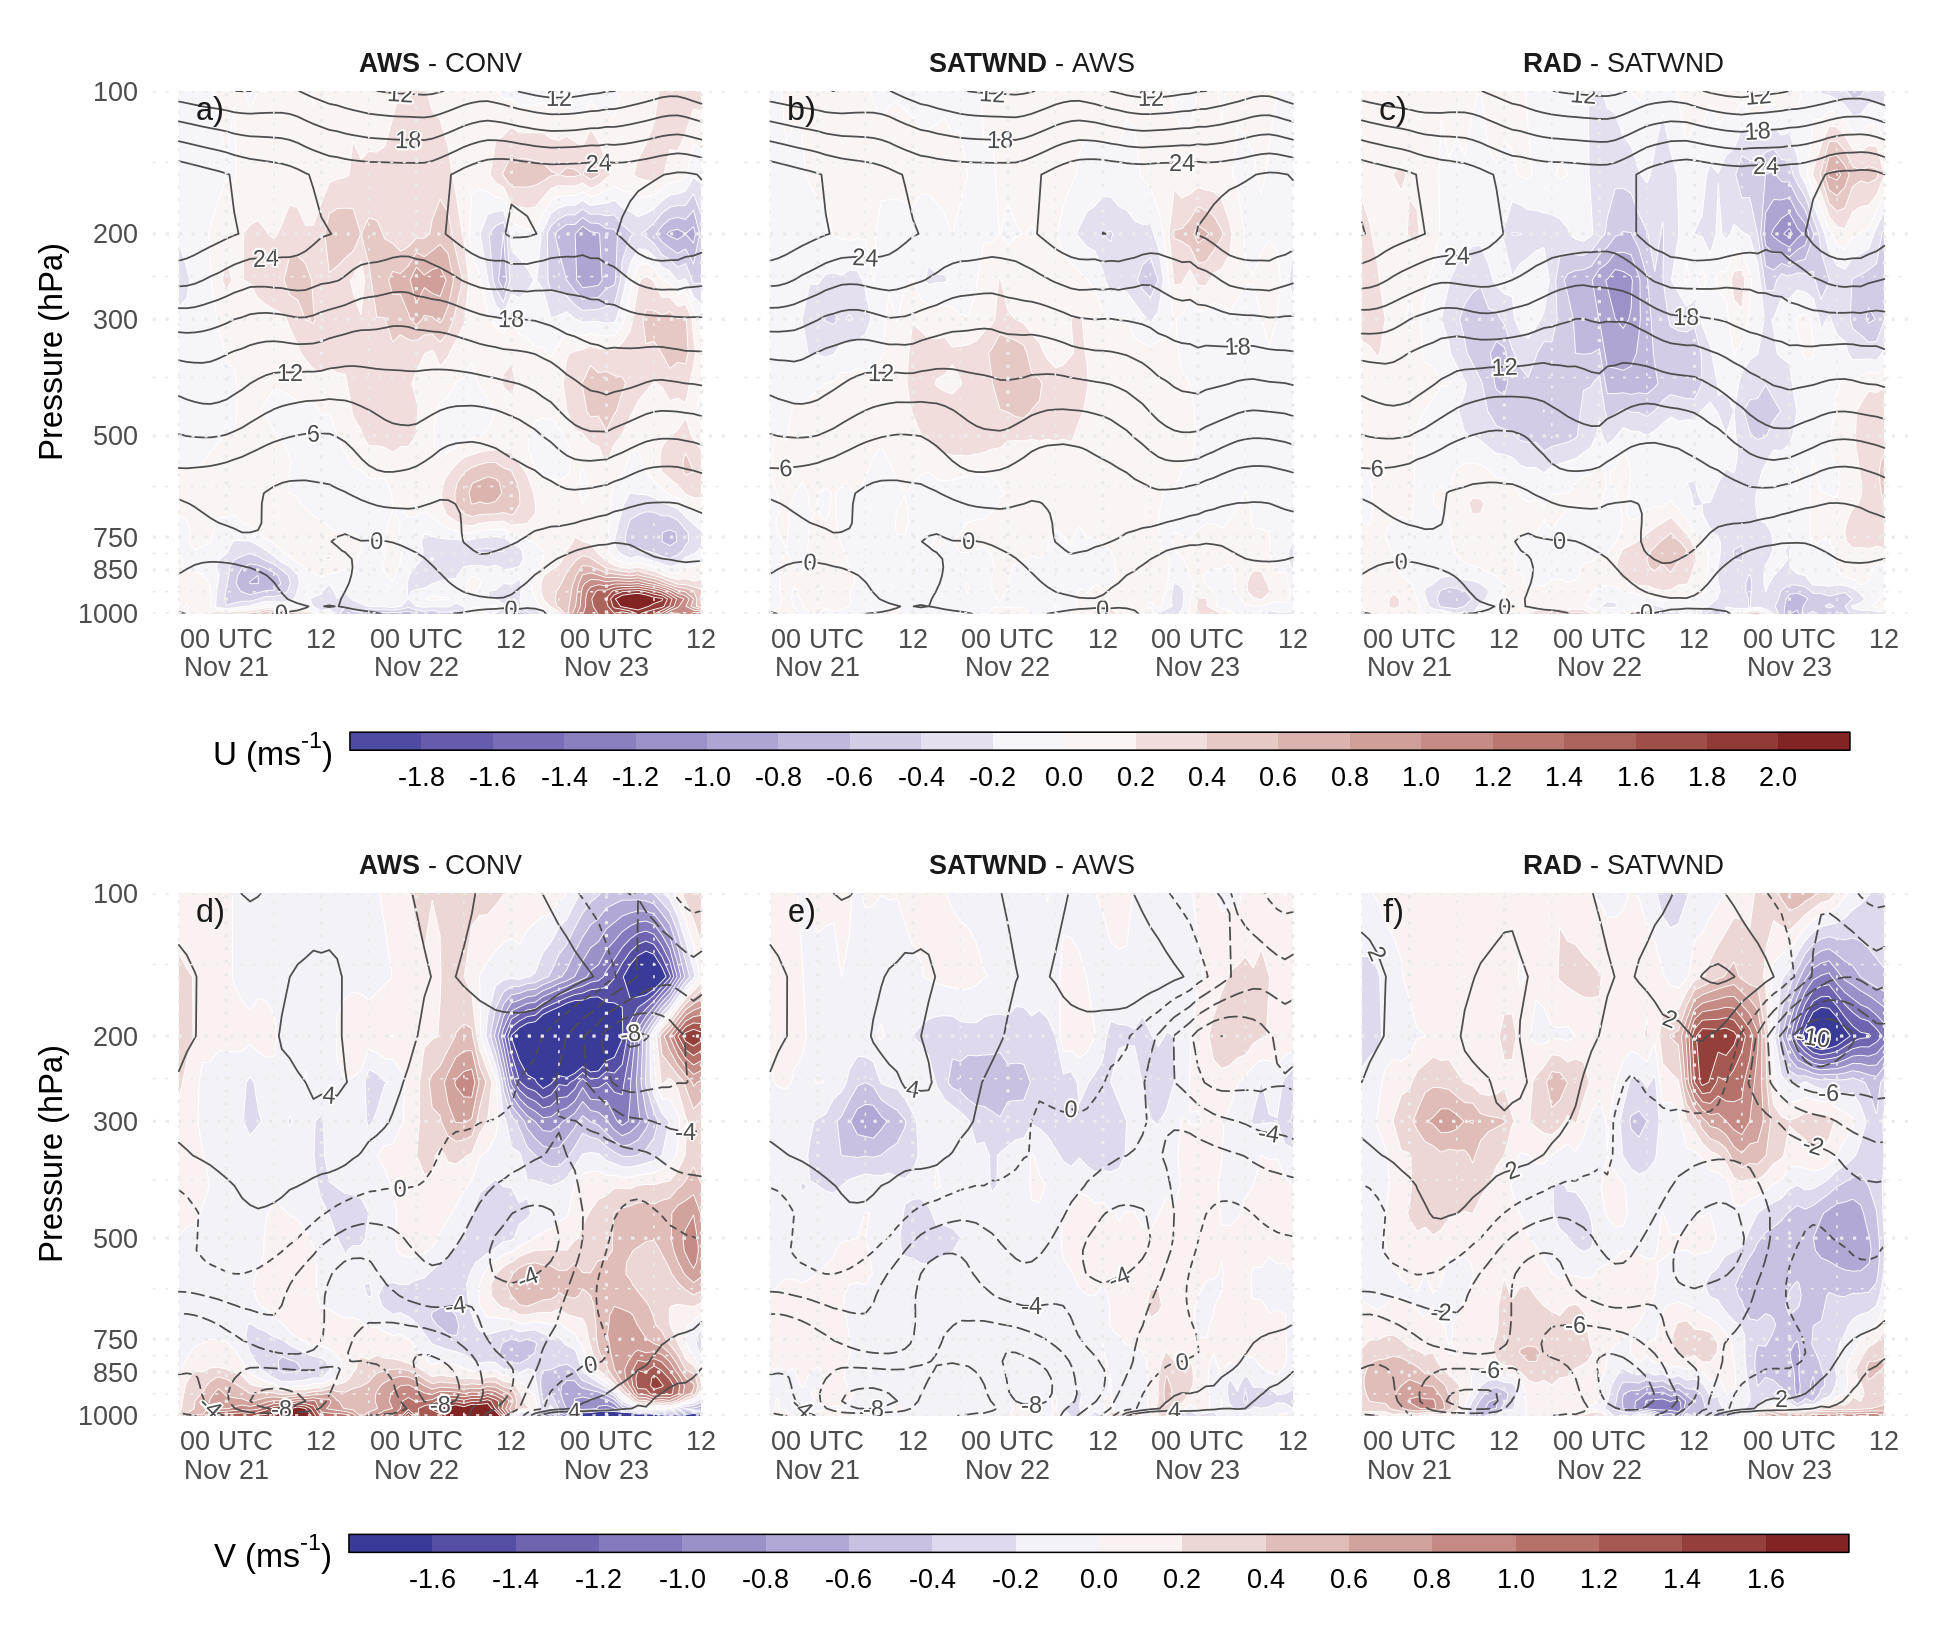
\includegraphics{../figures/UV-diff-1} 

}

\caption{Difference between analysis ensemble mean experiments a) and d) AWS-CONV, b) and e) SATWND-AWS, and c) and f) RAD-SATWND for the spatially averaged vertical profiles of u wind (a, b, and c, in \(ms^{-1}\)) and v wind (d, e, and f in \(ms^{-1}\)) calculated over the inner domain (red box in Figure \ref{fig:dominio}a) for each analysis cycle. Black contours correspond to negative u wind for (a) AWS, (b) SATWND, and (c) RAD and v wind for (d) AWS, (e) SATWND, and (f) RAD. Dashed contours correspond to negative v wind.}\label{fig:UV-diff}
\end{figure*}

To investigate how changes in the PBL can modify the pre-convective environment, we compare the horizontal distribution of the low level northerly flow (for the first 7 sigma levels), precipitable water, low level temperature, and CAPE for the analysis at 00 UTC Nov 22 (after 30 assimilation cycles). At that moment the first convective cells were developing over the southern region of the domain along the cold front. Figure \ref{fig:summary-fields}a shows the precipitable water (shaded) and the vertically averaged low-level meridional wind component (contours). We found that the moist tongue extending over the northern part of the domain is enhanced by the assimilation of denser surface observations. The moisture increase is particularly strong at the southern tip of this tongue, just ahead of the cold front where convection initiation was taking place. AWS and SATWND experiments are very similar, with values of precipitable water over 55 \(kgm^{-2}\) north of 30\(^{\circ}\)S and a similar vertical distribution of specific humidity (not shown). RAD has lower precipitable water content than AWS and SATWND, but higher than CONV. The distribution of moisture at low levels in RAD seems to be the result of the combination of the moistening effect of assimilating AWS -- partially compensated by the assimilation of radiance observations -- and a reduced meridional moisture transport due to the weaker northerly flow over the center of the domain compared to CONV.

The analyzed distribution of temperature and moisture in the PBL (Figure \ref{fig:summary-fields}b) resembles the characteristics observed in the temperature profiles (Figure \ref{fig:TQ-diff}a-c) where AWS produces a colder PBL than CONV while the PBL in RAD is warmer that SATWND. On average the PBL in AWS and SATWND is colder than in CONV, while RAD shows a warmer PBL than AWS due to the assimilation of radiance observations. Figure \ref{fig:summary-fields}c shows the most unstable convective available potential energy (MCAPE, shaded) and the 0 to 6 \(km\) wind shear. The values of MCAPE in CONV do not exceed 2000 \(JKg^{-1}\) while the rest of the experiments show maximum MCAPE over 4000 \(JKg^{-1}\). MCAPE in the RAD experiment is lower compared to AWS or SATWND. This is consistent with less humidity in the PBL with respect to these experiments but may be partially compensated by a slightly warmer PBL in the RAD experiment. The 0-6 km wind shear is more intense in AWS, SATWND, and RAD reaching values over 15 \(ms^{-1}\) at the southern tip of the region with positive MCAPE values. Moreover, in this same region, these experiments show larger MCAPE values than CONV. Note that wind shear over 15 \(ms^{-1}\) is associated with the development of more intense and organized MCSs (Chen et al., 2015) and also with conditions favorable for supercells (Markowski and Richardson, 2010).



\begin{figure*}
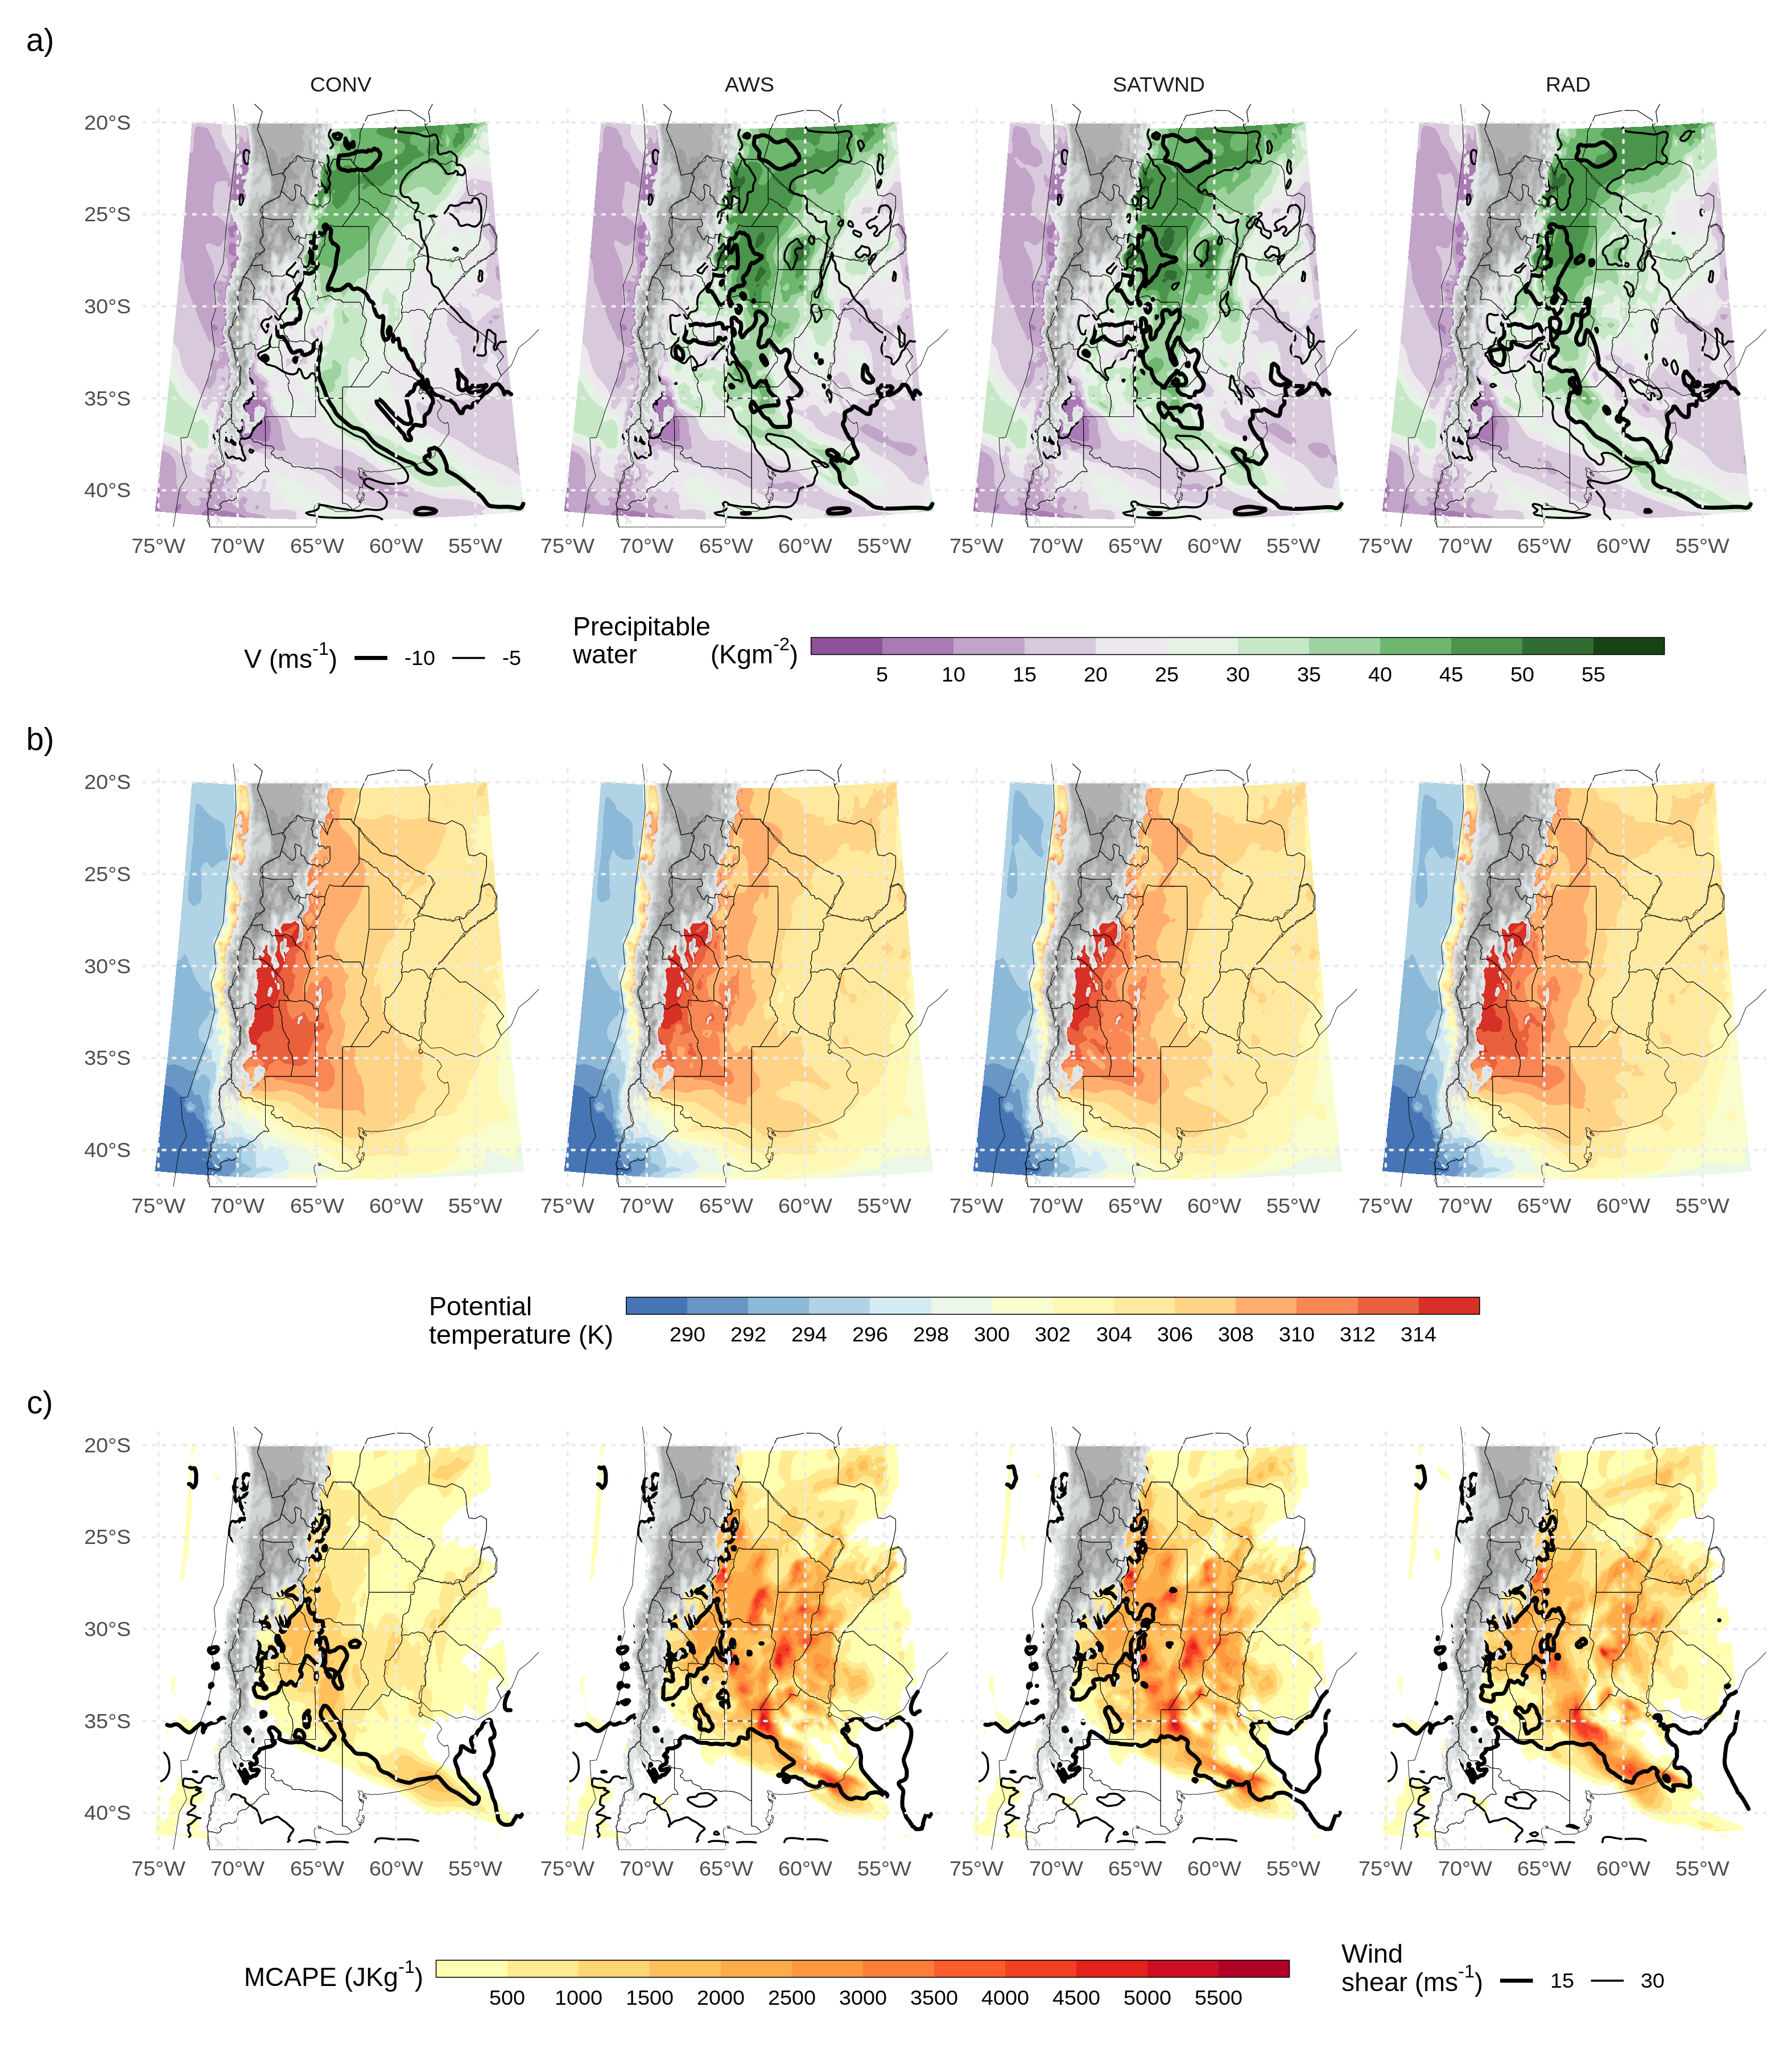
\includegraphics[width=1\linewidth]{../figures/summary-fields-1} \caption{a) Precipitable water (shaded, \(kgm^{-2}\)) and average northerly wind over the first 7 sigma levels (from the surface up to approximately 800 hPa, contours, \(ms^{-1}\)), b) Average potential temperature for the PBL (first 10 sigma levels), and c) Maximum CAPE and \textasciitilde0-6 km wind shear over 15 and 30 \(ms^{-1}\) for each experiment. All fields correspond to the analysis ensemble mean for 00 UTC Nov 22. Grey filled contours correspond to topography over 1500 meters above sea level.}\label{fig:summary-fields}
\end{figure*}

\hypertarget{validation-against-independent-observations}{%
\subsection{Validation against independent observations}\label{validation-against-independent-observations}}

First, we analyze the impact of assimilating different observation types in terms of the representation of the MCS and its associated precipitation. Figure \ref{fig:pp-hov}a shows the mean hourly accumulated precipitation as estimated by IMERG, and the probability matched mean (PM) (Clark, 2017) for the first-guess hourly accumulated precipitation as averaged between 67\(^{\circ}\)W and 54.5\(^{\circ}\)W as a function of time and latitude in the different experiments. The heaviest precipitation (over 12 \(mmh^{-1}\)) starts during the afternoon of Nov 22 and continues during Nov 23 after the end of the simulated period (Figure \ref{fig:pp-hov}a). In all the experiments, the accumulated precipitation in the short-range forecasts is underestimated. This is particularly evident in CONV (Figure \ref{fig:pp-hov}b), where the convection initiation is delayed and occurs further north with respect to the observed initiation. AWS, SATWND, and RAD better capture the timing and location of convective initiation (Figures \ref{fig:pp-hov}c-e). AWS and RAD show a more fragmented distribution compared with SATWND, possibly due to the development of less organized convection during Nov 22. After 18 UTC Nov 22, RAD shows improvements in the precipitation rate and its distribution compared to the other experiments as a result of enhanced development of the convection.



\begin{figure*}[h]
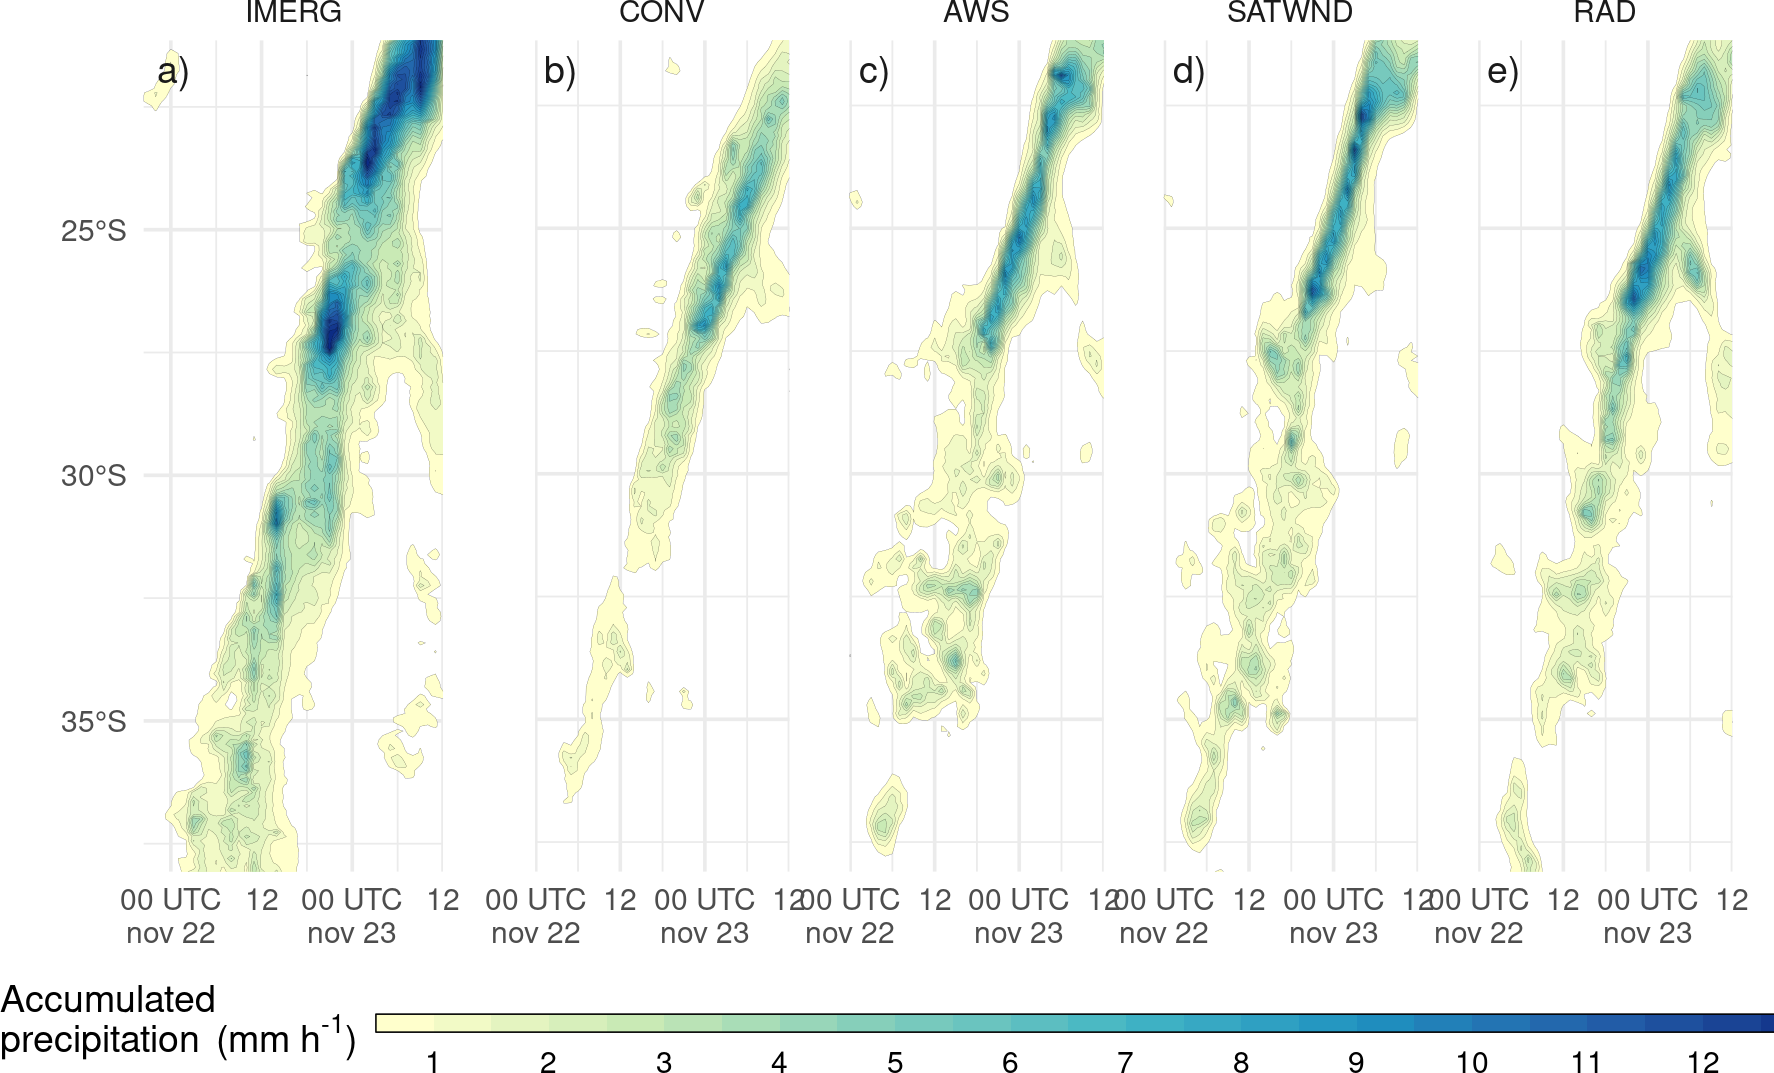
\includegraphics{../figures/pp-hov-1} \caption{Hövmoller diagram of probability matched mean hourly accumulated 1-h forecast precipitation for each latitude band estimated by IMERG (left) and simulated (right), for the ensemble mean of each experiment, averaged over a longitude range between 67\(^{\circ}\)W and 54.5\(^{\circ}\)W. Contours drawn every 0.5 \(mmh^{-1}\), starting at 0.5 \(mmh^{-1}\).}\label{fig:pp-hov}
\end{figure*}

To quantify the spatial match between the observed precipitation and the short-range forecast precipitation for the different experiments, we compute the FSS in 6-hour moving windows for different thresholds and spatial scales (Figure \ref{fig:fss}). All experiments show similar values of FSS during the initialization of the convection before 06 UTC Nov 22 except for RAD which performs better than the rest of the experiments during this period. This indicates that radiance observations have a positive impact on the analysis. The FSS for CONV is the lowest compared to the rest of the experiments and the differences are larger during the mature stage of the MCS. AWS and SATWND show similar FSSs indicating that satellite-derived wind assimilation has little impact on the precipitation for this case study. The assimilation of radiances led to an overall improvement of the 1-hour forecast precipitation, particularly for the 25 mm threshold during the period of heaviest precipitation on Nov 22 (Figure \ref{fig:fss}b,d). The enhancement is also important at the developing stage of the MCS (between 00 and 12 UTC Nov, 22 and also for spatial scales above 500 km, not shown).



\begin{figure}
\centering
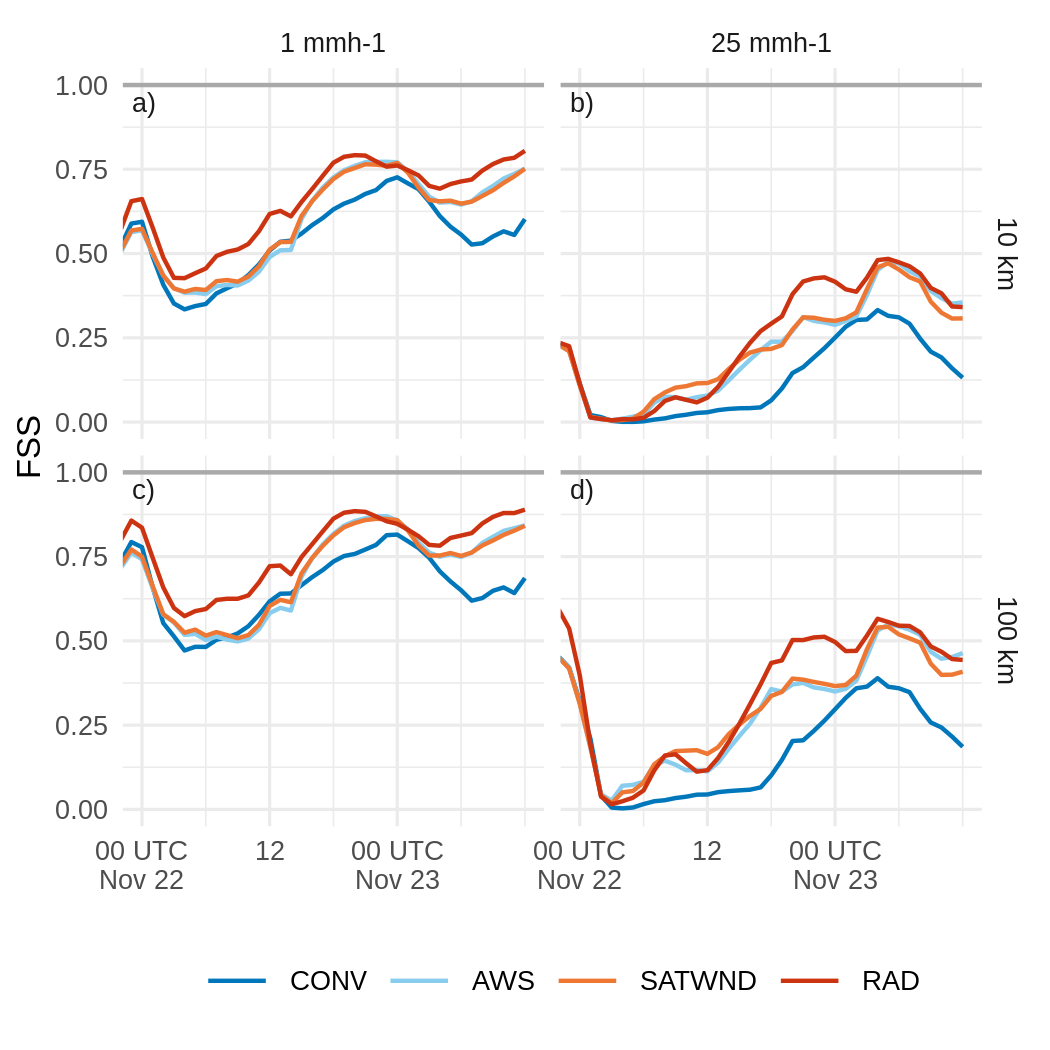
\includegraphics{../figures/fss-1.png}
\caption{\label{fig:fss}FSS calculated over 1-h forecast precipitation accumulated in a 6-hour moving window for 1 mm (a and c) and 25 mm (b and d) thresholds, on 10 km (a and b) and 100 km (c and d) scales, for the first-guess of CONV (blue line), AWS (light blue line), SATWND (orange line) and RAD (red line) experiments.}
\end{figure}

To complement the analysis, Figure \ref{fig:dbz-mean} shows the observed maximum reflectivity in the vertical column (COLMAX) and the ensemble mean COLMAX for the CONV and RAD experiments at different times between 10 and 19 UTC Nov 22. These experiments were chosen because they represent the analysis with the minimum (CONV) and maximum (RAD) number of assimilated observations. In addition, they are the worst (CONV) and best (RAD) performing experiments in terms of the 1-hour precipitation forecast skill (Figure \ref{fig:fss}). Overall, none of the short-range forecasts capture the mesoscale details in the reflectivity distribution. This is partially expected considering the coarse horizontal grid spacing (10 km), which is not enough to appropriately represent the strength of the convective band associated with the MCS. Also, the ensemble mean produces a smoothing effect that reduces the amplitude of local maxima in the forecast reflectivity field. RAD better represents the observed features of the system showing a stronger and more organized MCS than CONV, over the domain center at 10 and 13 UTC (first and second columns in Figure \ref{fig:dbz-mean}). The convective cells that initiate after 16 UTC along the warm front in the northeast part of the domain are well captured by both experiments but are better represented in terms of strength in RAD. In addition, CONV captures the location of the MCS, but the convection seems to be less organized and much weaker than in RAD. Before and after the times shown in Figure \ref{fig:dbz-mean}, the agreement between experiment and observations is quite good in the regions where radar data are available, especially for RAD.

Finally, Figure \ref{fig:soundings} shows the RMSE and bias calculated by comparing the experiments with radiosonde data from the RELAMPAGO missions, IOP 7 from 15 to 21 UTC Nov 21 (including 30 radiosondes), and IOP 8 from 14 to 20 UTC Nov 22 (including 22 radiosondes).

IOP 7 (Figures \ref{fig:soundings}a-d) provides a good characterization of the pre-convective environment during the first day of our experiments. The area where the observations were taken was characterized by mostly clear skies and a low-level northerly flow associated with warm and moist advection. In general, the experiments show a similar RMSE and bias for all the variables. AWS observations were able to reduce the RMSE for temperature and dew point temperature in the PBL and reduce a small dry bias. However, AWS degradated the zonal wind between 7 and 12 km increasing the bias and RMSE (Figure \ref{fig:soundings}c).



\begin{figure*}[h]
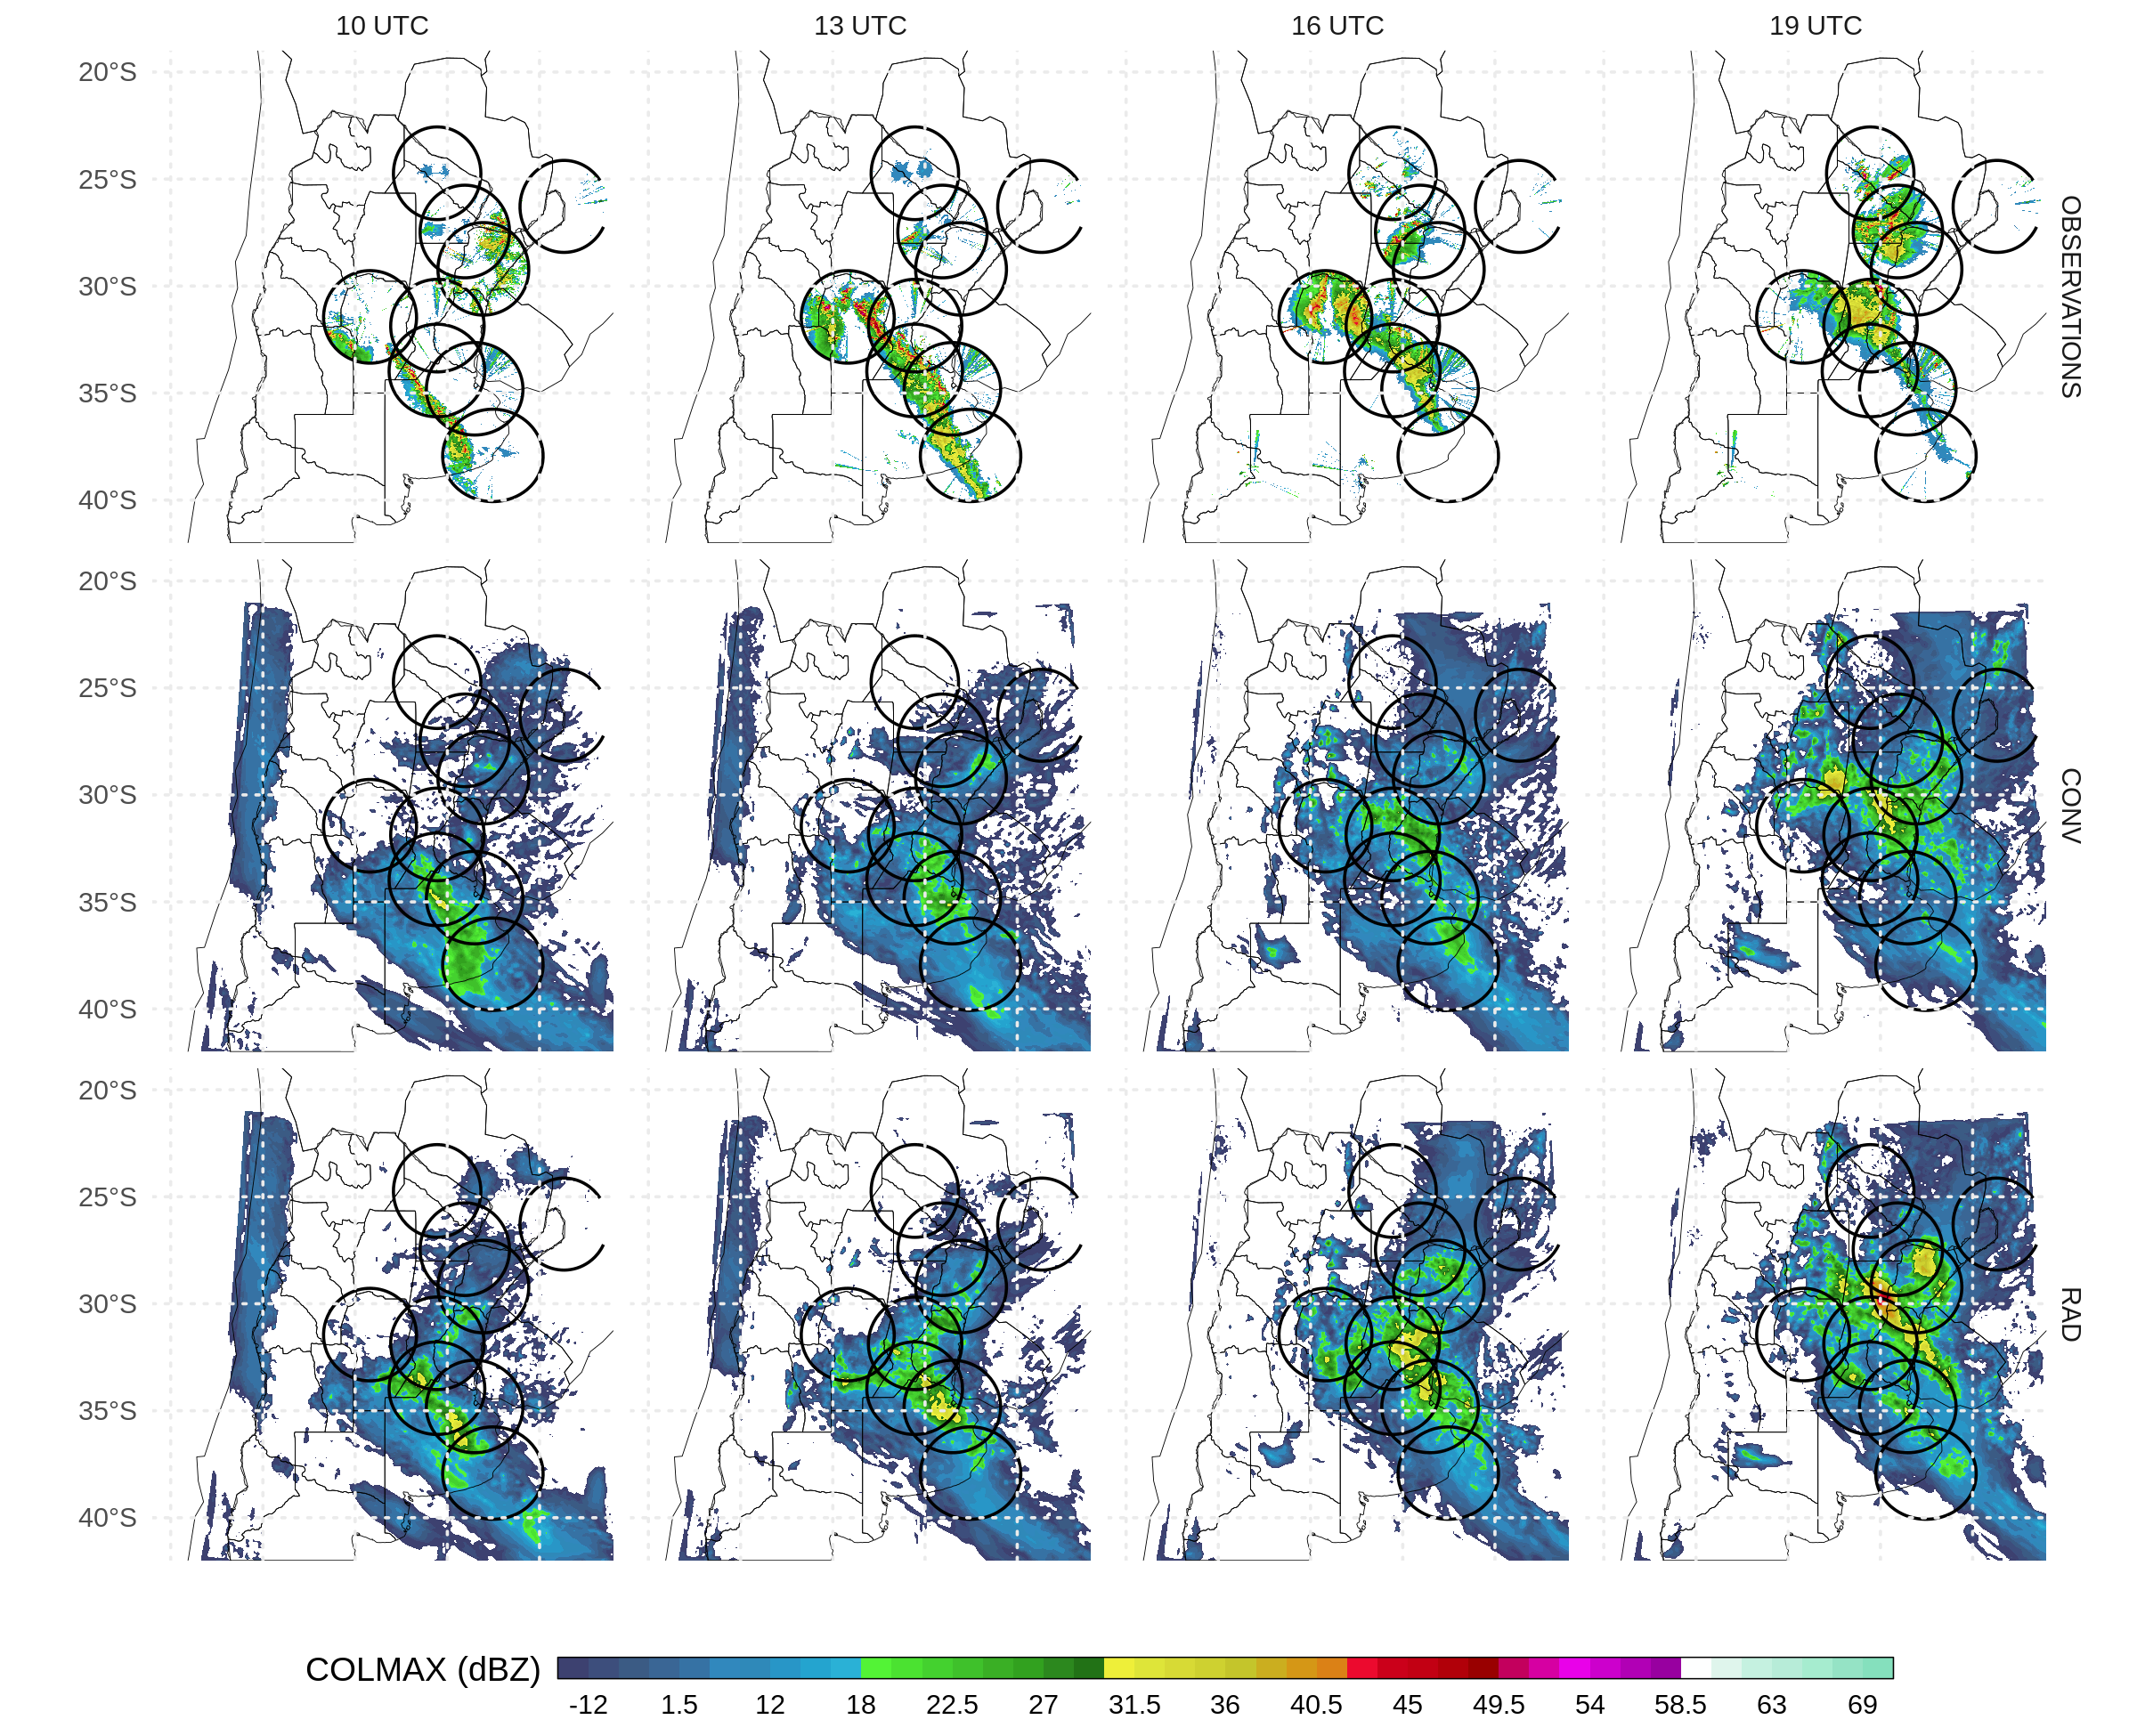
\includegraphics[width=1\linewidth]{../figures/dbz-mean-1} \caption{Maximum reflectivity in the column (COLMAX in \(dBZ\)), observed (upper row) and 1-hr forecast ensemble mean column maximum reflectivity for CONV (second row) and RAD (third row) at 10 UTC (first column), 13 UTC (second column), 16 UTC (third column), and 19 UTC (fourth column) Nov 22, 2018. Black circles in first row show the observation range of each radar.}\label{fig:dbz-mean}
\end{figure*}

For IOP 8 (Figures \ref{fig:soundings}e-h), the densely observed area was behind the MCS, but far enough from it to not be directly affected by its mesoscale circulation. This area was also behind the cold front and affected by low-level cold advection. The assimilation of AWS, SATWND, and RAD reduces the cold bias and RMSE for temperature between 5 and 12 km and the RMSE in the PBL compared with CONV (Figure \ref{fig:soundings}e). The reduction of bias and RMSE is also important for dew point temperature (Figure \ref{fig:soundings}f) with SATWND showing the bigger impact followed by AWS and RAD. The zonal wind is overestimated in the analyses and only RAD shows an improvement with respect to CONV in the upper troposphere (Figure \ref{fig:soundings}g). At low levels the meridional wind (Figure \ref{fig:soundings}g) presents a negative bias, indicating an underestimation of the southerly wind behind the cold front principally in AWS, SATWND, and RAD. In fact, low level biases in these experiments are higher than in the CONV experiment, indicating a detrimental effect of the additional observations (possibly associated with the effect of AWS).



\begin{figure*}[t]

{\centering 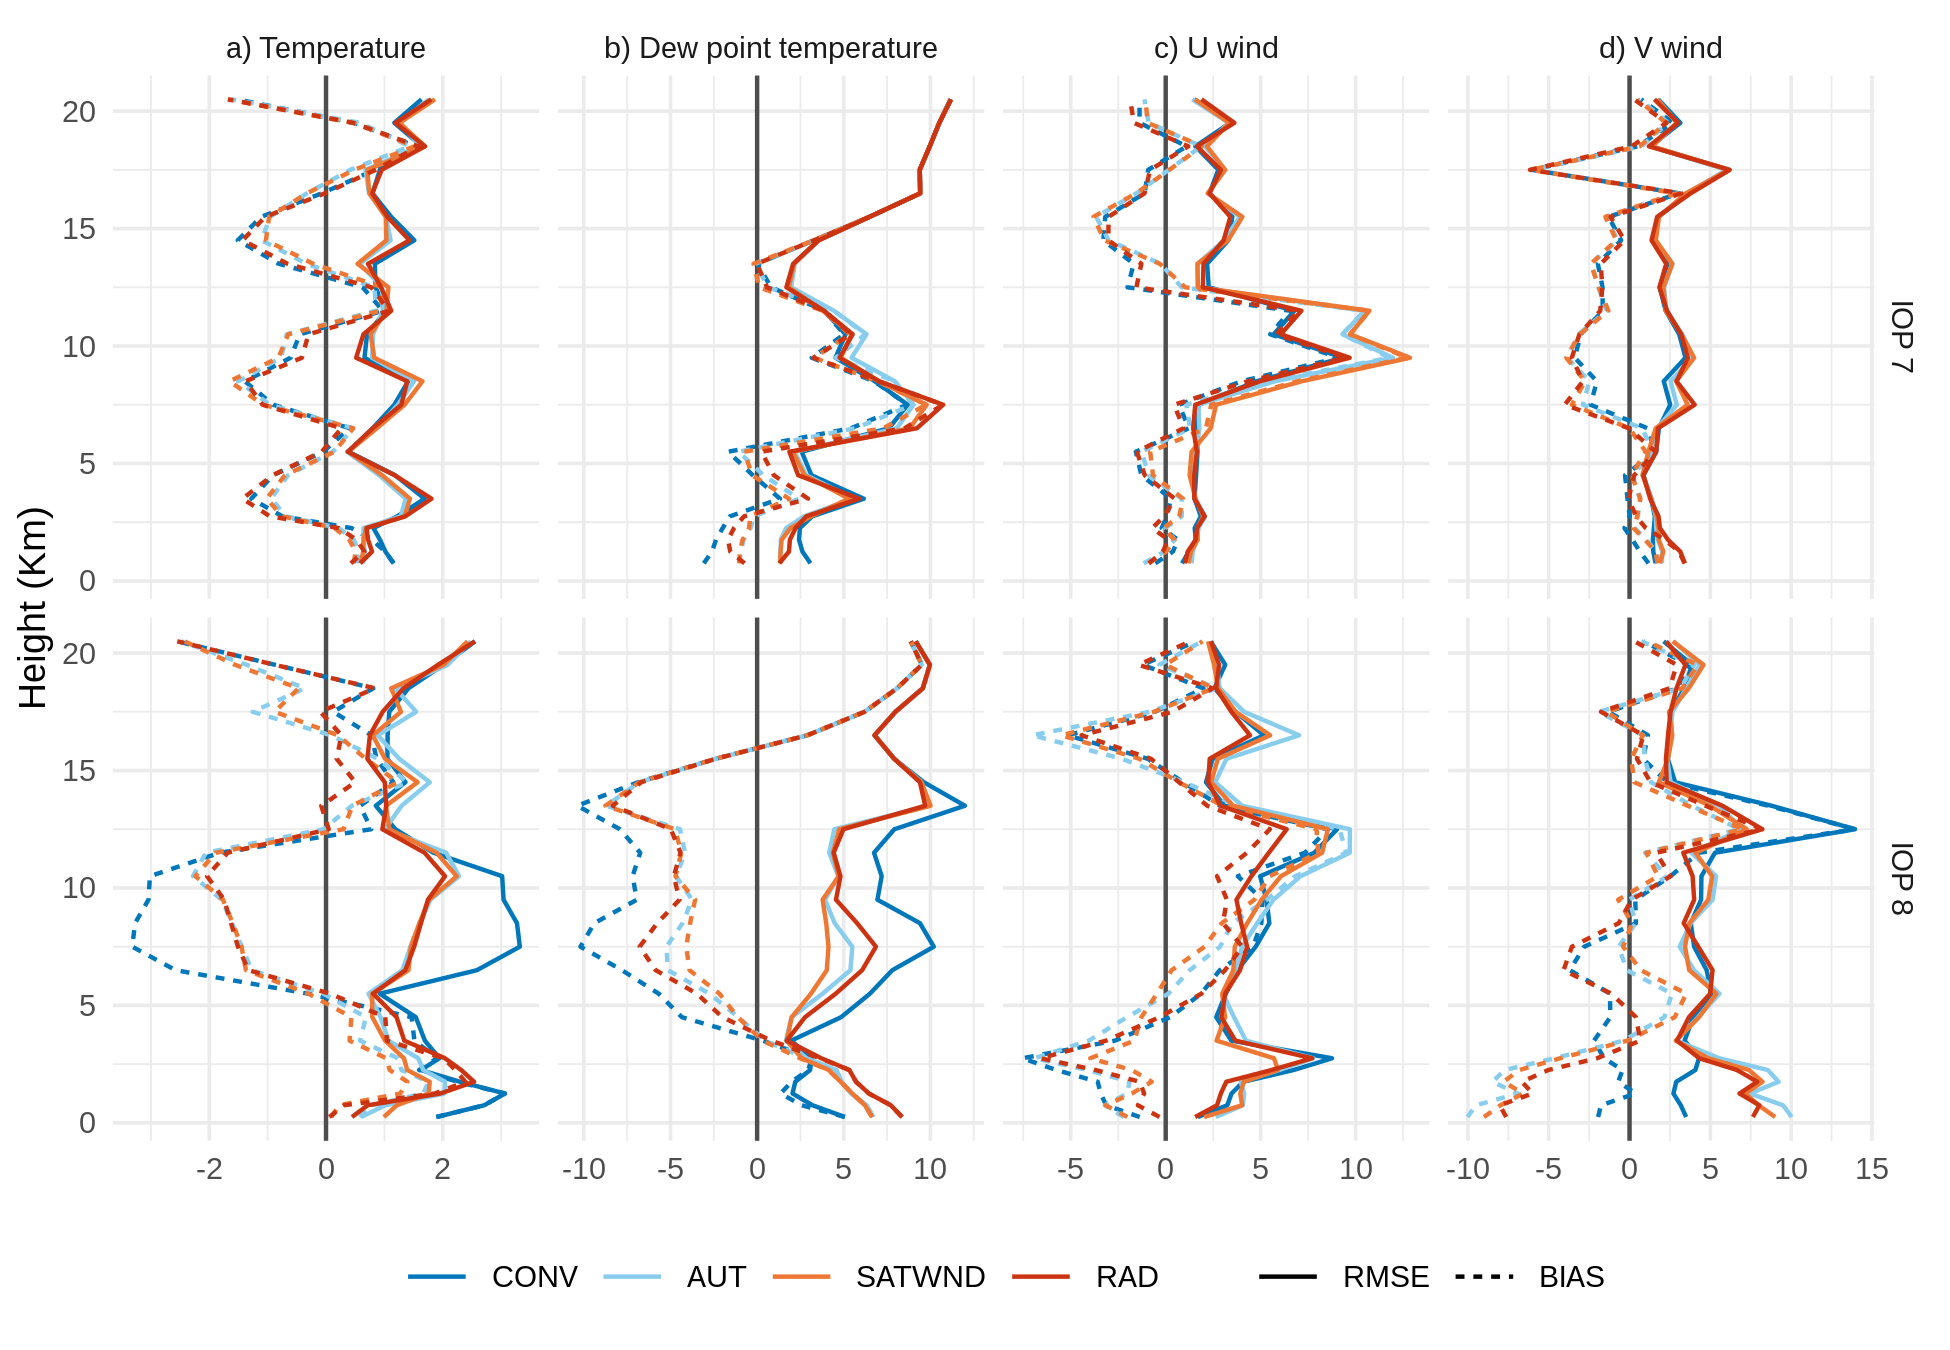
\includegraphics{../figures/soundings-1} 

}

\caption{RMSE (solid line) and Bias (dashed line) of a) temperature (\(K\)), b) dew point temperature (\(K\)), c) u wind (\(ms^{-1}\)) and d) v wind (\(ms^{-1}\)) calculated by comparing the analysis of each experiment with the RELAMPAGO soundings during IOP 7 and IOP 8. The blue line corresponds to CONV, the light blue line to AWS, SATWND is represented with an orange line, and RAD with a red line.}\label{fig:soundings}
\end{figure*}

\hypertarget{ensemble-forescast-validation}{%
\subsection{Ensemble forescast validation}\label{ensemble-forescast-validation}}

In this section, we analyze the 60-member ensemble forecast initialized at 00 and 06 UTC Nov 22 from each experiment. We calculated the FSS for the ensemble forecasts in 6-hour moving windows for the same thresholds and spatial scales as for the 1-h forecast to quantify the skill of the forecasts to predict precipitation (Figure \ref{fig:fssfcst}). CONV forecasts perform very poorly in terms of the FSS compared with the experiments that include other sources of observations. AWS, SATWND, and RAD show improvements in the FSS values, particularly for the higher threshold (Figure \ref{fig:fssfcst}b, d). Moreover, the late initialization at 06 UTC performs better for AWS, SATWND, and RAD tham the forecast initialized at 00 UTC, highlighting the positive impact of the observations assimilated between 00 and 06 UTC.

The satellite-derived wind observations show a clearly positive impact on the forecast, in contrast to what was seen when comparing the 1-h forecast with independent observations in terms of precipitation. Conversely, the radiance observations resulted in a neutral to a slightly negative impact on the forecast as opposed to what was seen when comparing the 1-h forecast to IMERG estimations.



\begin{figure}
\centering
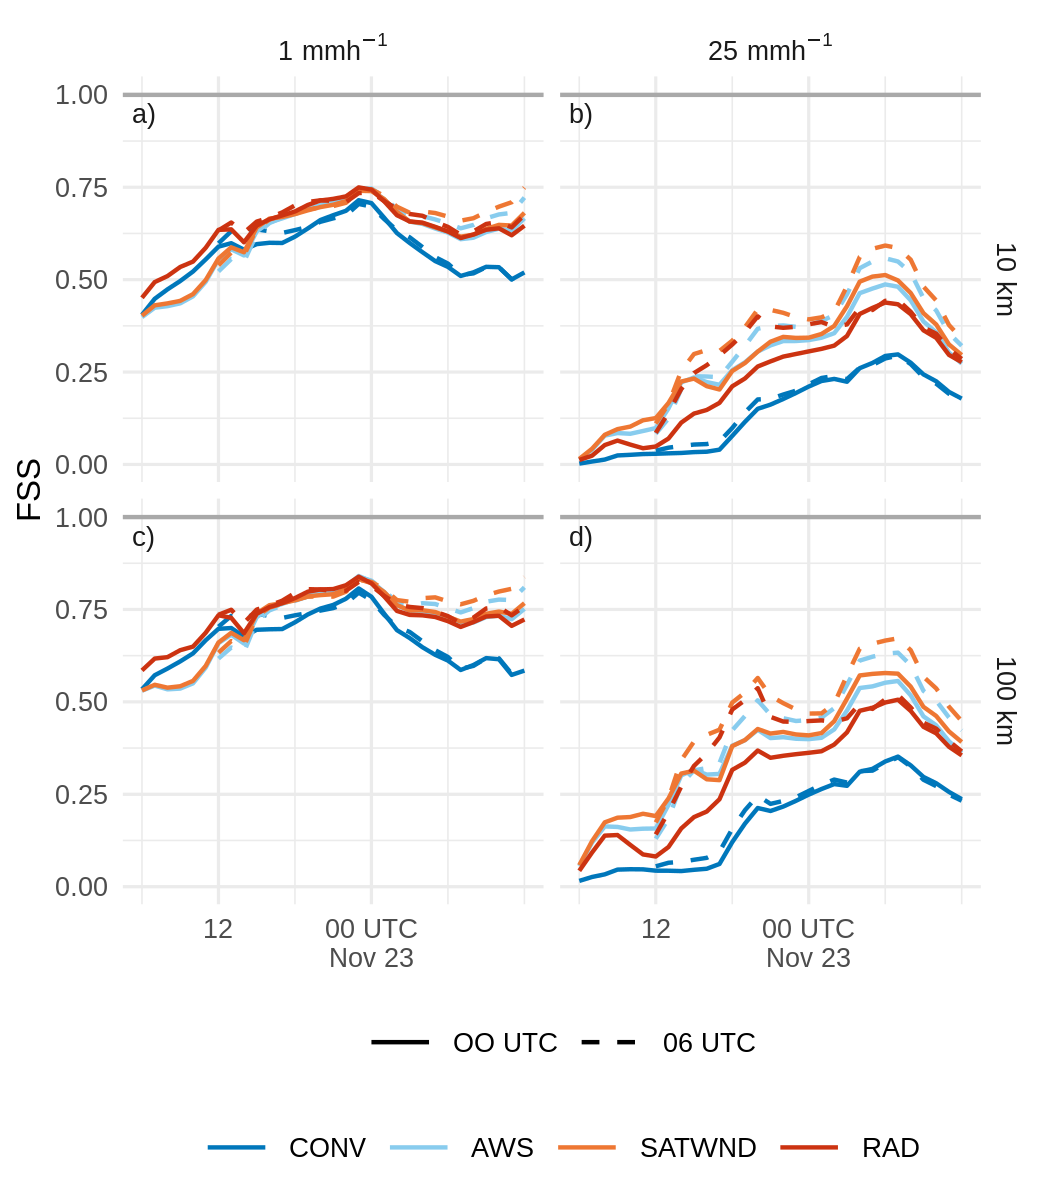
\includegraphics{../figures/fssfcst-1.png}
\caption{\label{fig:fssfcst}FSS calculated over a 6-hour moving window for 1 mm (a and c) and 25 mm (b and d) thresholds, on 10 km (a and b) and 100 km (c and d) scales, for the forecasts initialized from CONV (blue line), AWS (light blue line), SATWND (orange line), and RAD (red line) experiments at 00 UTC (solid line) and 06 UTC (dashed line), Nov 22.}
\end{figure}

\hypertarget{conclusions}{%
\section{Conclusions}\label{conclusions}}

In this paper, we investigate for the first time in South America the impact of different observation systems on the performance of an ensemble-based mesoscale regional DA system. In particular, we explore the impact upon the analysis quality of assimilating frequent and relatively dense surface observations, satellite derived winds, and satellite clear-sky radiances from multiple sensors. Southern South America is a particularly interesting region due to the heterogeneity and sometimes coarse resolution of the operational observing network (considering both surface based and upper air observations). This combined with a climatology characterized by frequent organized convective events makes mesoscale DA particularly challenging. To consider these issues, we used a case study approach of a massive mesoscale convective system that developed over Southern South America, particularly in a region where the surface and upper-air observing networks are too coarse to capture variability at the mesoscale and that took place on Nov 22, 2018.

We evaluated the consistency of the ensemble using the RCRV calculated for each type of observation used in RAD. Conventional observations including surface data and upper air observations from soundings and aircraft, show a \(sd RCRV\) near 1 indicating a good agreement between the ensemble spread and the observational errors with respect to the distance between the ensemble mean and the observations. For satellite-derived winds and radiance observations, the \(sd RCRV\) is lower than 1, which could be the result of an underdispersive ensemble or an overestimation of the observation errors. However, taking into account that the observation error for satellite-derived wind is overestimated (to avoid strong impacts on the analysis for poor quality estimations) and that the results obtained for more reliable observations (such as soundings) were good, we conclude that the ensemble has a reasonable spread.

In terms of the analysis, we found that AWS observations, which have high spatial and temporal resolution, produce impacts throughout the troposphere, especially in the PBL. In particular, the precipitable water content and the low level meridional circulation in the AWS experiment lead to the development of deep convection and heavy precipitation closer to the observed in this case study. We also found positive results when assimilating radiance observations that produce an adequate development of the convection, mainly during the mature stage of the MCS, leading to an increase in the accumulated precipitation compared with the other experiments. However, all experiments underestimated the 1-hour accumulated precipitation when compared to IMERG estimates. While the assimilation of satellite-derived wind does not produce a noticeable impact on the analysis with respect to the AWS experiment, this is possibly due to the small number of observations in low levels available for this case study and its large observation error. However, there are substantial improvements for the accumulated precipitation distribution. A more comprehensive analysis is necessary to assess the possible impacts on middle and upper levels.

Taking advantage of the observations taken during the RELAMPAGO field campaign, we compared the experiments with the soundings launched during IOPs 7 and 8. For the pre-convective environment (IOP 7), we observed an improvement at low levels when assimilating AWS observations for the temperature, dew point temperature, and meridional wind. In particular, AWS observations correct a dry bias already observed by Ruiz et al. (2010). For IOP 8, after the MCS crossed the center of the domain, we found a positive impact in low levels when assimilating more observations for the temperature but the opposite effect for the dew point temperature. In this case, the analyses have a moist bias that increases with the assimilation of AWS and radiance observations. We noted a negative covariance between temperature and moisture content over this region that could lead to a moistening of the PBL. It is not clear what produces these negative covariances but it is evident that the corrections introduced by the observations are degrading the estimation of the moisture content during this period, which requires further analysis.

We also analyzed the performance of independent ensemble forecasts intialized from the analyses to forecast the precipitation during Nov 22. The forecast initialized from AWS, SATWND, and RAD are able to forecast the precipitation substantially better than CONV. In particular, the continuous assimilation of satellite-derived wind and radiance observations helps to improve the latest initialization but only the satellite-derived wind observations produces a positive impact that persists throughout the forecast.

To summarize, in this study we conclude that the assimilation of surface observations with higher spatial and temporal resolution, satellite-derived winds, and clear-sky radiances from polar orbiting satellites had an overall positive impact on the development of the studied MCS and its associated precipitation. Moreover, the ensemble forecasts initialized from the analysis show promising results to predict the precipitation of severe events. In the future, we will further analyze the impacts in the independent forecasts and evaluate the implementation of other sources of observations like GPS radio occultation data and radiances from geostationary orbiting satellites.

\hypertarget{acknowledgements}{%
\section{Acknowledgements}\label{acknowledgements}}

We are very thankful to the Atmospheric and Sea Research Center (CIMA), the University of Buenos Aires (UBA), and the National Scientific and Technical Research Council (CONICET) who support this study. We acknowledge the Sistema Nacional de Radares Meteorológicos supported by the Secretaría de Infraestructura y Política Hídrica for kindly providing the radar observations used for validation and the National Meteorological Service for facilitating the access to the data. We also acknowledge the Cheyenne HPC resources (doi:10.5065/D6RX99HX) from NCAR's Computational and Information Systems Laboratory, National Science Foundation (project code UIUC0012). Also, PICT 2017-2233 and PICT 2018-3202 projects of the National Agency for the Promotion of Research, Technological Development and Innovation from Argentina partially funded this project.

\hypertarget{references}{%
\section*{References}\label{references}}
\addcontentsline{toc}{section}{References}

\hypertarget{refs}{}
\leavevmode\hypertarget{ref-allaire2019}{}%
Allaire, J., Horner, J., Xie, Y., Marti, V., Porte, N., 2019. Markdown: Render markdown with the c library 'sundown'.

\leavevmode\hypertarget{ref-bae2022}{}%
Bae, J.-H., Min, K.-H., 2022. Forecast Characteristics of Radar Data Assimilation Based on the Scales of Precipitation Systems. Remote Sensing 14, 605. doi:\href{https://doi.org/10.3390/rs14030605}{10.3390/rs14030605}

\leavevmode\hypertarget{ref-banos2021}{}%
Banos, I.H., Mayfield, W.D., Ge, G., Sapucci, L.F., Carley, J.R., Nance, L., 2021. Assessment of the data assimilation framework for the Rapid Refresh Forecast System v0.1 and impacts on forecasts of convective storms. Geoscientific Model Development Discussions 1--36. doi:\href{https://doi.org/10.5194/gmd-2021-289}{10.5194/gmd-2021-289}

\leavevmode\hypertarget{ref-bao2015}{}%
Bao, Y., Xu, J., Powell Jr., A.M., Shao, M., Min, J., Pan, Y., 2015. Impacts of AMSU-A, MHS and IASI data assimilation on temperature and humidity forecasts with GSI--WRF over the western United States. Atmos. Meas. Tech. 8, 4231--4242. doi:\href{https://doi.org/10.5194/amt-8-4231-2015}{10.5194/amt-8-4231-2015}

\leavevmode\hypertarget{ref-brooks2003}{}%
Brooks, H.E., Lee, J.W., Craven, J.P., 2003. The spatial distribution of severe thunderstorm and tornado environments from global reanalysis data. Atmospheric Research 67--68, 73--94. doi:\href{https://doi.org/10.1016/S0169-8095(03)00045-0}{10.1016/S0169-8095(03)00045-0}

\leavevmode\hypertarget{ref-campitelli2020}{}%
Campitelli, E., 2020. metR: Tools for Easier Analysis of Meteorological Fields.

\leavevmode\hypertarget{ref-candille2007}{}%
Candille, G., Côté, C., Houtekamer, P.L., Pellerin, G., 2007. Verification of an Ensemble Prediction System against Observations. Mon. Wea. Rev. 135, 2688--2699. doi:\href{https://doi.org/10.1175/MWR3414.1}{10.1175/MWR3414.1}

\leavevmode\hypertarget{ref-cecil2012}{}%
Cecil, D.J., Blankenship, C.B., 2012. Toward a Global Climatology of Severe Hailstorms as Estimated by Satellite Passive Microwave Imagers. Journal of Climate 25, 687--703. doi:\href{https://doi.org/10.1175/JCLI-D-11-00130.1}{10.1175/JCLI-D-11-00130.1}

\leavevmode\hypertarget{ref-chang2017}{}%
Chang, W., Jacques, D., Fillion, L., Baek, S.-J., 2017. Assimilation of Hourly Surface Observations with the Canadian High-Resolution Ensemble Kalman Filter. Atmosphere-Ocean 55, 247--263. doi:\href{https://doi.org/10.1080/07055900.2017.1384361}{10.1080/07055900.2017.1384361}

\leavevmode\hypertarget{ref-chen2001}{}%
Chen, F., Dudhia, J., 2001. Coupling an Advanced Land Surface--Hydrology Model with the Penn State--NCAR MM5 Modeling System. Part I: Model Implementation and Sensitivity. Monthly Weather Review 129, 569--585. doi:\href{https://doi.org/10.1175/1520-0493(2001)129\%3C0569:CAALSH\%3E2.0.CO;2}{10.1175/1520-0493(2001)129\textless0569:CAALSH\textgreater2.0.CO;2}

\leavevmode\hypertarget{ref-chen2015}{}%
Chen, Q., Fan, J., Hagos, S., Gustafson, W.I., Berg, L.K., 2015. Roles of wind shear at different vertical levels: Cloud system organization and properties. Journal of Geophysical Research: Atmospheres 120, 6551--6574. doi:\href{https://doi.org/10.1002/2015JD023253}{10.1002/2015JD023253}

\leavevmode\hypertarget{ref-chen2016}{}%
Chen, X., Zhao, K., Sun, J., Zhou, B., Lee, W.-C., 2016. Assimilating surface observations in a four-dimensional variational Doppler radar data assimilation system to improve the analysis and forecast of a squall line case. Adv. Atmos. Sci. 33, 1106--1119. doi:\href{https://doi.org/10.1007/s00376-016-5290-0}{10.1007/s00376-016-5290-0}

\leavevmode\hypertarget{ref-cherubini2006}{}%
Cherubini, T., Businger, S., Velden, C., Ogasawara, R., 2006. The Impact of Satellite-Derived Atmospheric Motion Vectors on Mesoscale Forecasts over Hawaii. Monthly Weather Review 134, 2009--2020. doi:\href{https://doi.org/10.1175/MWR3163.1}{10.1175/MWR3163.1}

\leavevmode\hypertarget{ref-clark2017}{}%
Clark, A.J., 2017. Generation of Ensemble Mean Precipitation Forecasts from Convection-Allowing Ensembles. Weather and Forecasting 32, 1569--1583. doi:\href{https://doi.org/10.1175/WAF-D-16-0199.1}{10.1175/WAF-D-16-0199.1}

\leavevmode\hypertarget{ref-Cheyenne2019}{}%
Computational and Information Systems Laboratory, 2019. Cheyenne: HPE/SGI ICE XA System (University Community Computing). National Center for Atmospheric Research Boulder, CO. doi:\href{https://doi.org/doi:10.5065/D6RX99HX}{doi:10.5065/D6RX99HX}

\leavevmode\hypertarget{ref-deelia2017}{}%
de Elía, R., Vidal, L., Lohigorry, P., 2017. El SMN y la red argentina de radares meteorológicos {[}WWW Document{]}. URL \url{http://hdl.handle.net/20.500.12160/625}

\leavevmode\hypertarget{ref-dillon2021}{}%
Dillon, M.E., Maldonado, P., Corrales, P., Skabar, Y.G., Ruiz, J., Sacco, M., Cutraro, F., Mingari, L., Matsudo, C., Vidal, L., Rugna, M., Hobouchian, M.P., Salio, P., Nesbitt, S., Saulo, C., Kalnay, E., Miyoshi, T., 2021. A rapid refresh ensemble based data assimilation and forecast system for the RELAMPAGO field campaign. Atmospheric Research 105858. doi:\href{https://doi.org/10.1016/j.atmosres.2021.105858}{10.1016/j.atmosres.2021.105858}

\leavevmode\hypertarget{ref-dillon2016}{}%
Dillon, M.E., Skabar, Y.G., Ruiz, J., Kalnay, E., Collini, E.A., Echevarría, P., Saucedo, M., Miyoshi, T., Kunii, M., 2016. Application of the WRF-LETKF Data Assimilation System over Southern South America: Sensitivity to Model Physics. Wea. Forecasting 31, 217--236. doi:\href{https://doi.org/10.1175/WAF-D-14-00157.1}{10.1175/WAF-D-14-00157.1}

\leavevmode\hypertarget{ref-dowle2020}{}%
Dowle, M., Srinivasan, A., 2020. Data.Table: Extension of 'data.frame'.

\leavevmode\hypertarget{ref-sondeos}{}%
Earth Observing Laboratory, U. -, 2020. Multi-network composite highest resolution radiosonde data. Version 1.3. UCAR/NCAR - earth observing laboratory.

\leavevmode\hypertarget{ref-eyre2020}{}%
Eyre, J.R., English, S.J., Forsythe, M., 2020. Assimilation of satellite data in numerical weather prediction. Part I: The early years. Quarterly Journal of the Royal Meteorological Society 146, 49--68. doi:\href{https://doi.org/10.1002/qj.3654}{10.1002/qj.3654}

\leavevmode\hypertarget{ref-garcia2019}{}%
Garcia, F., Ruiz, J., Salio, P., Bechis, H., Nesbitt, S., 2019. Argentina mesonet data. Version 1.1. UCAR/NCAR - earth observing laboratory.

\leavevmode\hypertarget{ref-gasperoni2018}{}%
Gasperoni, N.A., Wang, X., Brewster, K.A., Carr, F.H., 2018. Assessing Impacts of the High-Frequency Assimilation of Surface Observations for the Forecast of Convection Initiation on 3 April 2014 within the Dallas--Fort Worth Test Bed. Monthly Weather Review 146, 3845--3872. doi:\href{https://doi.org/10.1175/MWR-D-18-0177.1}{10.1175/MWR-D-18-0177.1}

\leavevmode\hypertarget{ref-grell2013}{}%
Grell, G.A., Freitas, S.R., 2013. A scale and aerosol aware stochastic convective parameterization for weather and air quality modeling. Atmos. Chem. Phys. Discuss. 13, 23845--23893. doi:\href{https://doi.org/10.5194/acpd-13-23845-2013}{10.5194/acpd-13-23845-2013}

\leavevmode\hypertarget{ref-goncalvesdegoncalves2015}{}%
gustavo Goncalves de Goncalves, L., Sapucci, L., Vendrasco, E., de Mattos, J.G., Ferreira, C., Khamis, E., Cruz, N., 2015. A rapid update data assimilation cycle over South America using 3DVar and EnKF, in: The 20th International TOVS Study Conference (ITSC-20). The 20th International TOVS Study Conference (ITSC-20), Lake Geneva, Wisconsin, USA.

\leavevmode\hypertarget{ref-ha2014}{}%
Ha, S.-Y., Snyder, C., 2014. Influence of Surface Observations in Mesoscale Data Assimilation Using an Ensemble Kalman Filter. Monthly Weather Review 142, 1489--1508. doi:\href{https://doi.org/10.1175/MWR-D-13-00108.1}{10.1175/MWR-D-13-00108.1}

\leavevmode\hypertarget{ref-han2006}{}%
Han, Y., Van Delst, P., Liu, Q., Weng, F., Yan, B., Treadon, R., Derber, J., 2006. JCSDA Community Radiative Transfer Model (CRTM)---version 1, NOAA Technical Report NESDIS 122. Washington, D.C.

\leavevmode\hypertarget{ref-hong2006a}{}%
Hong, S.-Y., Kim, J.-H., Lim, J.-o., Dudhia, J., 2006. The WRF Single Moment 6-Class Microphysics Scheme (WSM6). Journal of the Korean Meteorological Society 42, 129--151.

\leavevmode\hypertarget{ref-hong2006}{}%
Hong, S.-Y., Noh, Y., Dudhia, J., 2006. A New Vertical Diffusion Package with an Explicit Treatment of Entrainment Processes. Mon. Wea. Rev. 134, 2318--2341. doi:\href{https://doi.org/10.1175/MWR3199.1}{10.1175/MWR3199.1}

\leavevmode\hypertarget{ref-hu2018}{}%
Hu, M., Ge, G., Zhou, C., Stark, D., Shao, H., Newman, K., Beck, J., Zhang, X., 2018. Grid-point Statistical Interpolation (GSI) User's Guide Version 3.7. Developmental Testbed Center.

\leavevmode\hypertarget{ref-huffman2018}{}%
Huffman, G., Bolvin, D., Braithwaite, D., Hsu, K., Joyce, R., Kidd, C., Nelkin, E., Sorooshian, S., Tan, J., Xie, P., 2018. NASA Global Precipitation Measurement (GPM) Integrated Multi-satellitE Retrievals for GPM (IMERG). National Aeronautics and Space Administration (NASA).

\leavevmode\hypertarget{ref-hunt2007}{}%
Hunt, B.R., Kostelich, E.J., Szunyogh, I., 2007. Efficient data assimilation for spatiotemporal chaos: A local ensemble transform Kalman filter. Physica D: Nonlinear Phenomena 230, 112--126. doi:\href{https://doi.org/10.1016/j.physd.2006.11.008}{10.1016/j.physd.2006.11.008}

\leavevmode\hypertarget{ref-iacono2008}{}%
Iacono, M.J., Delamere, J.S., Mlawer, E.J., Shephard, M.W., Clough, S.A., Collins, W.D., 2008. Radiative forcing by long-lived greenhouse gases: Calculations with the AER radiative transfer models. J. Geophys. Res. 113, D13103. doi:\href{https://doi.org/10.1029/2008JD009944}{10.1029/2008JD009944}

\leavevmode\hypertarget{ref-janjic1994}{}%
Janjić, Z.I., 1994. The Step-Mountain Eta Coordinate Model: Further Developments of the Convection, Viscous Sublayer, and Turbulence Closure Schemes. Mon. Wea. Rev. 122, 927--945. doi:\href{https://doi.org/10.1175/1520-0493(1994)122\%3C0927:TSMECM\%3E2.0.CO;2}{10.1175/1520-0493(1994)122\textless0927:TSMECM\textgreater2.0.CO;2}

\leavevmode\hypertarget{ref-jones2013}{}%
Jones, T.A., Otkin, J.A., Stensrud, D.J., Knopfmeier, K., 2013. Assimilation of Satellite Infrared Radiances and Doppler Radar Observations during a Cool Season Observing System Simulation Experiment. Mon. Wea. Rev. 141, 3273--3299. doi:\href{https://doi.org/10.1175/MWR-D-12-00267.1}{10.1175/MWR-D-12-00267.1}

\leavevmode\hypertarget{ref-kain2004}{}%
Kain, J.S., 2004. The Kain--Fritsch Convective Parameterization: An Update. JOURNAL OF APPLIED METEOROLOGY 43, 12.

\leavevmode\hypertarget{ref-lin2017a}{}%
Lin, H., Weygandt, S.S., Benjamin, S.G., Hu, M., 2017. Satellite Radiance Data Assimilation within the Hourly Updated Rapid Refresh. Wea. Forecasting 32, 1273--1287. doi:\href{https://doi.org/10.1175/WAF-D-16-0215.1}{10.1175/WAF-D-16-0215.1}

\leavevmode\hypertarget{ref-maejima2019}{}%
Maejima, Y., Miyoshi, T., Kunii, M., Seko, H., Sato, K., 2019. Impact of Dense and Frequent Surface Observations on 1-Minute-Update Severe Rainstorm Prediction: A Simulation Study. Journal of the Meteorological Society of Japan. Ser. II 97, 253--273. doi:\href{https://doi.org/10.2151/jmsj.2019-014}{10.2151/jmsj.2019-014}

\leavevmode\hypertarget{ref-maldonado2021}{}%
Maldonado, P., Ruiz, J., Saulo, C., 2021. Sensitivity to Initial and Boundary Perturbations in Convective-Scale Ensemble-Based Data Assimilation: Imperfect-Model OSSEs. SOLA 17, 96--102. doi:\href{https://doi.org/10.2151/sola.2021-015}{10.2151/sola.2021-015}

\leavevmode\hypertarget{ref-mallick2020}{}%
Mallick, S., Jones, T.A., 2020. Assimilation of GOES-16 satellite derived winds into the warn-on-forecast system. Atmospheric Research 245, 105131. doi:\href{https://doi.org/10.1016/j.atmosres.2020.105131}{10.1016/j.atmosres.2020.105131}

\leavevmode\hypertarget{ref-markowski2010}{}%
Markowski, P., Richardson, Y., 2010. Organization of Isolated Convection, in: Mesoscale Meteorology in Midlatitudes. John Wiley \& Sons, Ltd, pp. 201--244. doi:\href{https://doi.org/10.1002/9780470682104.ch8}{10.1002/9780470682104.ch8}

\leavevmode\hypertarget{ref-matsudo2015}{}%
Matsudo, C., García Skabar, Y., Ruiz, J., Vidal, L., Salio, P., 2015. Verification of WRF-ARW convective-resolving forecasts over Southeastern South America. Mausam 66, 445--456.

\leavevmode\hypertarget{ref-nakanishi2009}{}%
Nakanishi, M., Niino, H., 2009. Development of an Improved Turbulence Closure Model for the Atmospheric Boundary Layer. JMSJ 87, 895--912. doi:\href{https://doi.org/10.2151/jmsj.87.895}{10.2151/jmsj.87.895}

\leavevmode\hypertarget{ref-cisl_rda_ds084.1}{}%
National Centers for Environmental Prediction, National Weather Service, NOAA, U.S. Department of Commerce, 2015. NCEP GFS 0.25 degree global forecast grids historical archive.

\leavevmode\hypertarget{ref-necker2020}{}%
Necker, T., Geiss, S., Weissmann, M., Ruiz, J., Miyoshi, T., Lien, G., 2020. A convective‐scale 1,000‐member ensemble simulation and potential applications. Q.J.R. Meteorol. Soc 146, 1423--1442. doi:\href{https://doi.org/10.1002/qj.3744}{10.1002/qj.3744}

\leavevmode\hypertarget{ref-nesbitt2021}{}%
Nesbitt, S.W., Salio, P.V., Ávila, E., Bitzer, P., Carey, L., Chandrasekar, V., Deierling, W., Dominguez, F., Dillon, M.E., Garcia, C.M., Gochis, D., Goodman, S., Hence, D.A., Kosiba, K.A., Kumjian, M.R., Lang, T., Luna, L.M., Marquis, J., Marshall, R., McMurdie, L.A., Nascimento, E.L., Rasmussen, K.L., Roberts, R., Rowe, A.K., Ruiz, J.J., Sabbas, E.F.M.T.S., Saulo, A.C., Schumacher, R.S., Skabar, Y.G., Machado, L.A.T., Trapp, R.J., Varble, A., Wilson, J., Wurman, J., Zipser, E.J., Arias, I., Bechis, H., Grover, M.A., 2021. A storm safari in Subtropical South America: Proyecto RELAMPAGO. Bulletin of the American Meteorological Society -1, 1--64. doi:\href{https://doi.org/10.1175/BAMS-D-20-0029.1}{10.1175/BAMS-D-20-0029.1}

\leavevmode\hypertarget{ref-otsuka2015}{}%
Otsuka, M., Kunii, M., Seko, H., Shimoji, K., Hayashi, M., Yamashita, K., 2015. Assimilation Experiments of MTSAT Rapid Scan Atmospheric Motion Vectors on a Heavy Rainfall Event. Journal of the Meteorological Society of Japan. Ser. II 93, 459--475. doi:\href{https://doi.org/10.2151/jmsj.2015-030}{10.2151/jmsj.2015-030}

\leavevmode\hypertarget{ref-ouaraini2015}{}%
Ouaraini, R.E., Berre, L., Fischer, C., Sayouty, E.H., 2015. Sensitivity of regional ensemble data assimilation spread to perturbations of lateral boundary conditions. Tellus A: Dynamic Meteorology and Oceanography 67, 28502. doi:\href{https://doi.org/10.3402/tellusa.v67.28502}{10.3402/tellusa.v67.28502}

\leavevmode\hypertarget{ref-rasmussen2014}{}%
Rasmussen, K.L., Zuluaga, M.D., Houze, R.A., 2014. Severe convection and lightning in subtropical South America. Geophysical Research Letters 41, 7359--7366. doi:\href{https://doi.org/10.1002/2014GL061767}{10.1002/2014GL061767}

\leavevmode\hypertarget{ref-rcoreteam2020}{}%
R Core Team, 2020. R: A language and environment for statistical computing. R Foundation for Statistical Computing, Vienna, Austria.

\leavevmode\hypertarget{ref-roberts2008}{}%
Roberts, N., 2008. Assessing the spatial and temporal variation in the skill of precipitation forecasts from an NWP model. Meteorological Applications 15, 163--169. doi:\href{https://doi.org/10.1002/met.57}{10.1002/met.57}

\leavevmode\hypertarget{ref-ruiz2010}{}%
Ruiz, J.J., Saulo, C., Nogués-Paegle, J., 2010. WRF Model Sensitivity to Choice of Parameterization over South America: Validation against Surface Variables. Mon. Wea. Rev. 138, 3342--3355. doi:\href{https://doi.org/10.1175/2010MWR3358.1}{10.1175/2010MWR3358.1}

\leavevmode\hypertarget{ref-sawada2019}{}%
Sawada, M., Ma, Z., Mehra, A., Tallapragada, V., Oyama, R., Shimoji, K., 2019. Impacts of Assimilating High-Resolution Atmospheric Motion Vectors Derived from Himawari-8 on Tropical Cyclone Forecast in HWRF. Monthly Weather Review 147, 3721--3740. doi:\href{https://doi.org/10.1175/MWR-D-18-0261.1}{10.1175/MWR-D-18-0261.1}

\leavevmode\hypertarget{ref-shao2016}{}%
Shao, H., Derber, J., Huang, X.-Y., Hu, M., Newman, K., Stark, D., Lueken, M., Zhou, C., Nance, L., Kuo, Y.-H., Brown, B., 2016. Bridging Research to Operations Transitions: Status and Plans of Community GSI. Bulletin of the American Meteorological Society 97, 1427--1440. doi:\href{https://doi.org/10.1175/BAMS-D-13-00245.1}{10.1175/BAMS-D-13-00245.1}

\leavevmode\hypertarget{ref-singh2016}{}%
Singh, R., Ojha, S.P., Kishtawal, C.M., Pal, P.K., Kiran Kumar, A.S., 2016. Impact of the assimilation of INSAT-3D radiances on short-range weather forecasts: Assimilation of INSAT-3D Radiances. Q.J.R. Meteorol. Soc. 142, 120--131. doi:\href{https://doi.org/10.1002/qj.2636}{10.1002/qj.2636}

\leavevmode\hypertarget{ref-skamarock2008}{}%
Skamarock, W.C., Klemp, J.B., Dudhia, J., Gill, D.O., Barker, D.M., Duda, M.G., Huang, X.-Y., Wang, W., Powers, J.G., 2008. A Description of the Advanced Research WRF Version 3.

\leavevmode\hypertarget{ref-sobash2015}{}%
Sobash, R.A., Stensrud, D.J., 2015. Assimilating Surface Mesonet Observations with the EnKF to Improve Ensemble Forecasts of Convection Initiation on 29 May 2012. Monthly Weather Review 143, 3700--3725. doi:\href{https://doi.org/10.1175/MWR-D-14-00126.1}{10.1175/MWR-D-14-00126.1}

\leavevmode\hypertarget{ref-sun2014}{}%
Sun, J., Xue, M., Wilson, J.W., Zawadzki, I., Ballard, S.P., Onvlee-Hooimeyer, J., Joe, P., Barker, D.M., Li, P.-W., Golding, B., Xu, M., Pinto, J., 2014. Use of NWP for Nowcasting Convective Precipitation: Recent Progress and Challenges. Bulletin of the American Meteorological Society 95, 409--426. doi:\href{https://doi.org/10.1175/BAMS-D-11-00263.1}{10.1175/BAMS-D-11-00263.1}

\leavevmode\hypertarget{ref-wang2021}{}%
Wang, Z.Q., Randriamampianina, R., 2021. The Impact of Assimilating Satellite Radiance Observations in the Copernicus European Regional Reanalysis (CERRA). Remote Sensing 13, 426. doi:\href{https://doi.org/10.3390/rs13030426}{10.3390/rs13030426}

\leavevmode\hypertarget{ref-weston2019}{}%
Weston, P., Geer, A., Bormann, N., Bormann, N., 2019. Investigations into the assimilation of AMSU-A in the presence of cloud and precipitation {[}WWW Document{]}. EUMETSAT/ECMWF Fellowship Programme Research Report. doi:\href{https://doi.org/10.21957/ewahn9ce}{10.21957/ewahn9ce}

\leavevmode\hypertarget{ref-wheatley2010}{}%
Wheatley, D.M., Stensrud, D.J., 2010. The Impact of Assimilating Surface Pressure Observations on Severe Weather Events in a WRF Mesoscale Ensemble System. Monthly Weather Review 138, 1673--1694. doi:\href{https://doi.org/10.1175/2009MWR3042.1}{10.1175/2009MWR3042.1}

\leavevmode\hypertarget{ref-whitaker2012}{}%
Whitaker, J.S., Hamill, T.M., 2012. Evaluating Methods to Account for System Errors in Ensemble Data Assimilation. Mon. Wea. Rev. 140, 3078--3089. doi:\href{https://doi.org/10.1175/MWR-D-11-00276.1}{10.1175/MWR-D-11-00276.1}

\leavevmode\hypertarget{ref-wickham2009}{}%
Wickham, H., 2009. Ggplot2: Elegant Graphics for Data Analysis, Use R! Springer-Verlag, New York. doi:\href{https://doi.org/10.1007/978-0-387-98141-3}{10.1007/978-0-387-98141-3}

\leavevmode\hypertarget{ref-wu2014}{}%
Wu, T.-C., Liu, H., Majumdar, S.J., Velden, C.S., Anderson, J.L., 2014. Influence of Assimilating Satellite-Derived Atmospheric Motion Vector Observations on Numerical Analyses and Forecasts of Tropical Cyclone Track and Intensity. Monthly Weather Review 142, 49--71. doi:\href{https://doi.org/10.1175/MWR-D-13-00023.1}{10.1175/MWR-D-13-00023.1}

\leavevmode\hypertarget{ref-xie2015}{}%
Xie, Y., 2015. Dynamic documents with R and knitr, Second. ed. Chapman and Hall/CRC, Boca Raton, Florida.

\leavevmode\hypertarget{ref-zhao2021}{}%
Zhao, J., Gao, J., Jones, T.A., Hu, J., 2021a. Impact of Assimilating High-Resolution Atmospheric Motion Vectors on Convective Scale Short-Term Forecasts: 1. Observing System Simulation Experiment (OSSE). Journal of Advances in Modeling Earth Systems 13, e2021MS002484. doi:\href{https://doi.org/10.1029/2021MS002484}{10.1029/2021MS002484}

\leavevmode\hypertarget{ref-zhao2021a}{}%
Zhao, J., Gao, J., Jones, T.A., Hu, J., 2021b. Impact of Assimilating High-Resolution Atmospheric Motion Vectors on Convective Scale Short-Term Forecasts: 2. Assimilation Experiments of GOES-16 Satellite Derived Winds. Journal of Advances in Modeling Earth Systems 13, e2021MS002486. doi:\href{https://doi.org/10.1029/2021MS002486}{10.1029/2021MS002486}

\leavevmode\hypertarget{ref-zhu2019}{}%
Zhu, K., Xue, M., Pan, Y., Hu, M., Benjamin, S.G., Weygandt, S.S., Lin, H., 2019. The Impact of Satellite Radiance Data Assimilation within a Frequently Updated Regional Forecast System Using a GSI-based Ensemble Kalman Filter. Adv. Atmos. Sci. 36, 1308--1326. doi:\href{https://doi.org/10.1007/s00376-019-9011-3}{10.1007/s00376-019-9011-3}

\leavevmode\hypertarget{ref-zhu2014}{}%
Zhu, Y., Derber, J., Collard, A., Dee, D., Treadon, R., Gayno, G., Jung, J.A., 2014. Enhanced radiance bias correction in the National Centers for Environmental Prediction's Gridpoint Statistical Interpolation data assimilation system. Quarterly Journal of the Royal Meteorological Society 140, 1479--1492. doi:\href{https://doi.org/10.1002/qj.2233}{10.1002/qj.2233}

\leavevmode\hypertarget{ref-zhu2016}{}%
Zhu, Y., Liu, E., Mahajan, R., Thomas, C., Groff, D., Van Delst, P., Collard, A., Kleist, D., Treadon, R., Derber, J.C., 2016. All-Sky Microwave Radiance Assimilation in NCEP's GSI Analysis System. Mon. Wea. Rev. 144, 4709--4735. doi:\href{https://doi.org/10.1175/MWR-D-15-0445.1}{10.1175/MWR-D-15-0445.1}


\end{document}


